% !TeX program = xelatex
% !TeX encoding = UTF-8
% !TeX spellcheck = en_US
% !BIB program = biber
%% 
%% The above lines help editors like TeXstudio to automatically choose the right tools
%% to compile your LaTeX source file. If your tool does not support these magic comments,
%% you will need to make appropriate manual choices.
%% 
%% You can safely use "pdflatex" instead of "xelatex" if you prefer the pdfLaTeX toolchain.
%% However, pdfLaTeX will not be able to deliver the professional font experience that you
%% will get with XeLaTeX. You can also safely use "lualatex" instead of "xelatex" while
%% preserving the professional font experience if you prefer the LuaLaTeX toolchain.
%% 
%% _Important_: These magic comments should be on the first lines of your source file.
%% 
%%%%%%%%%%%%%%%%%%%%%%%%%%%%%%%%%%%%%%%%%%%%%%%%%%%%%%%%%%%%%%%%%%%%%%%%%%%%%%%%

%%%%%%%%%%%%%%%%%%%%%%%%%%%%%%%%%%%%%%%%%%%%%%%%%%%%%%%%%%%%%%%%%%%%%%%%%%%%%%%%
%% 
%%            JJJJ   K                         K   UUUU         UUUU  
%%            JJJJ   KKKK                   KKKK   UUUU         UUUU  
%%            JJJJ   KKKKKK               KKKKKK   UUUU         UUUU  
%%            JJJJ      KKKKKK         KKKKKK      UUUU         UUUU  
%%            JJJJ         KKKKKK   KKKKKK         UUUU         UUUU  
%%            JJJJ            KKKKKKKKK            UUUU         UUUU  
%%    JJ     JJJJJ               KKK               UUUUU       UUUUU  
%%  JJJJJJJJJJJJJ    KKKKKKKKKKKKKKKKKKKKKKKKKKK    UUUUUUUUUUUUUUU   
%%    JJJJJJJJJ      KKKKKKKKKKKKKKKKKKKKKKKKKKK      UUUUUUUUUUU     
%% 
%% This is an example file for using the JKU LaTeX technical report template
%% for your technical report.
%% 
%% Template created by Michael Roland (2021)
%% 
%%%%%%%%%%%%%%%%%%%%%%%%%%%%%%%%%%%%%%%%%%%%%%%%%%%%%%%%%%%%%%%%%%%%%%%%%%%%%%%%

%%%%%%%%%%%%%%%%%%%%%%%%%%%%%%%%%%%%%%%%%%%%%%%%%%%%%%%%%%%%%%%%%%%%%%%%%%%%%%%%
%% 
%% Document class: This is a koma-script article.
%% 
\documentclass[a4paper,oneside,11pt,ngerman]{scrartcl}
%% 
%% The comma-separated list in square brackets are class options.
%% Useful options that you might want to use:
%% 
%% Paper size:
%%  * a4paper ... A4 paper size
%% 
%% Optimize for single-sided or double-sided printing:
%%  * oneside ... single-sided
%%  * twoside ... double-sided
%% 
%% Base font size:
%%  * 10pt ... 10-pt font is used for normal text
%%  * 11pt ... 11-pt font is used for normal text
%% 
%% Define document languages (the last specified language becomes the document default
%% language):
%%  * ngerman ... German
%%  * english ... English
%%  * ...
%% 
%% Alternate document classes: The JKU report template supports the koma-script classes
%% `scrartcl', `scrreprt' and `scrbook'. The article class `scrartcl' is well-suited
%% for a typical technical report. However, `scrbook' or `scrreprt' may be better
%% suited for longer reports since they permit structuring your work in chapters.
%%  
%% _Important_: The document class should be the first line of LaTeX code in your main
%% source file. Do not place anything but comments / magic comments above that line (unless
%% you really know what you are doing).
%% 
%%%%%%%%%%%%%%%%%%%%%%%%%%%%%%%%%%%%%%%%%%%%%%%%%%%%%%%%%%%%%%%%%%%%%%%%%%%%%%%%

%%%%%%%%%%%%%%%%%%%%%%%%%%%%%%%%%%%%%%%%%%%%%%%%%%%%%%%%%%%%%%%%%%%%%%%%%%%%%%%%
%% 
%% Treat input files as UTF-8 encoded. Make sure to always load this when you use pdfLaTeX
%% so that pdfLaTeX knows how to read and interpret characters in this source file.
%% 
\usepackage[utf8]{inputenc}
%% 
%%%%%%%%%%%%%%%%%%%%%%%%%%%%%%%%%%%%%%%%%%%%%%%%%%%%%%%%%%%%%%%%%%%%%%%%%%%%%%%%

%%%%%%%%%%%%%%%%%%%%%%%%%%%%%%%%%%%%%%%%%%%%%%%%%%%%%%%%%%%%%%%%%%%%%%%%%%%%%%%%
%% 
%% Use the JKU LaTeX technical report template for this document.
%% 
\usepackage[
	TNF,
	techreport,
	fancyfonts,
	equalmargins,
	fontpath=../../assets/fonts,
	logopath=../../assets/logos
]{jkureport}
%% 
%% The comma-separated list in square brackets are theme options. Useful options that you
%% might want to use:
%% 
%% Document type:
%%  * phdthesis     ... PhD thesis.
%%  * mathesis      ... Master's thesis.
%%  * diplomathesis ... Diploma thesis.
%%  * bathesis      ... Bachelor's thesis.
%%  * seminarreport ... Seminar report.
%%  * techreport    ... Technical report.
%% 
%% Color scheme selection options:
%%  * JKU  ... Use JKU (gray) color scheme (this is the default if no scheme is selected).
%%  * BUS  ... Use Business School color scheme.
%%  * LIT  ... Use Linz Institute of Technology color scheme.
%%  * MED  ... Use MED faculty color scheme.
%%  * RE   ... Use RE faculty color scheme.
%%  * SOE  ... Use School of Education color scheme.
%%  * SOWI ... Use SOWI faculty color scheme.
%%  * TNF  ... Use TNF faculty color scheme.
%% 
%% Space-efficient monospace font options (requires XeTeX/LuaTeX):
%%  * compactmono   ... Use condensed fixed-width font everywhere.
%%  * nocompactverb ... Do not use condensed fixed-width font for verbatim and listings.
%% 
%% Style-breaking options:
%%  * noimprint      ... Do not insert imprint on title pages.
%%  * nojkulogo      ... Do not insert JKU & K logos on title pages.
%%  * capstitle      ... Set document title in capital letters.
%%  * nofancyfonts   ... Do not use custom TTF fonts with XeTeX/LuaTeX / supress pdfLaTeX warning.
%%  * equalmargins   ... Decrease the outer page margin to have both page margins of equal size
%%                       (the additional outer margin is intentional and to be used for
%%                       anotations; equalmargins also causes the text width to be
%%                       significantly larger than optimal for reading).
%% 
%% Experimental options:
%%  * mathastext ... Use standard document fonts (enhanced with symbols from Fira Math font
%%                   when using XeTeX/LuaTeX) in math mode.
%% 
%% Advanced options:
%%  * noautopdfinfo     ... Do not automatically try to add pdfinfo with hyperref from document
%%                          metadata fields.
%%  * logopath={<path>} ... Set the path where the theme can find its own logo resources. This
%%                          should typically be a relative path and the default is `./logos'.
%%  * fontpath={<path>} ... Set the path where the theme can find its own font resources. This
%%                          should typically be a relative path and the default is `./fonts'.
%% 
%% Hint: Boolean options can be used in the forms `option' or `option=true' the enable the
%% option and `nooption' or `option=false' to disable the option.
%% 
%%%%%%%%%%%%%%%%%%%%%%%%%%%%%%%%%%%%%%%%%%%%%%%%%%%%%%%%%%%%%%%%%%%%%%%%%%%%%%%%

%%%%%%%%%%%%%%%%%%%%%%%%%%%%%%%%%%%%%%%%%%%%%%%%%%%%%%%%%%%%%%%%%%%%%%%%%%%%%%%%
%% 
%% This is the place where you can load additional packages. If you want to load
%% a package `biblatex', you would use the command `\usepackage{biblatex}'.
%% 

\usepackage{amsfonts}
\usepackage{subfigure}
\usepackage{pdfpages}
\usepackage[european, straightvoltages]{circuitikz}
\usepackage{marginnote}
\usepackage{wrapfig}
\usepackage{ragged2e}
\usepackage{caption}
\usepackage{siunitx}
\usepackage{tabularx}
\usepackage{pgfplotstable}
\usepackage{enumitem}

% faster images
\graphicspath{{images_optimized/}{images/}}

% % tikz cache
% \usepackage{tikz}
% \usetikzlibrary{external}
% \tikzexternalize[prefix=tikz-cache/]

\setcounter{tocdepth}{2}

\tikzset{vmeter/.style={rmeterwa, t=V}}
\tikzset{ameter/.style={rmeterwa, t=A}}
\tikzset{ometer/.style={rmeterwa, t=$\Omega$}}

\renewcaptionname{ngerman}{\figurename}{Abb.}
\captionsetup{font=small}

\newcommand{\marginref}[1]{%
\reversemarginpar\marginnote{\textbf{(#1)}}[7pt]
}

\newcolumntype{Y}{>{\centering\arraybackslash}X}

%% 
%%%%%%%%%%%%%%%%%%%%%%%%%%%%%%%%%%%%%%%%%%%%%%%%%%%%%%%%%%%%%%%%%%%%%%%%%%%%%%%%

\begin{document}

\title{Messung grundlegender elektrischer Größen}
\author{Simon Grundner (k12136610) \and Paul Kronegger (k12344729)}
\setbottommark{Paul Kronegger (k12344729), Simon Grundner (k12136610)}

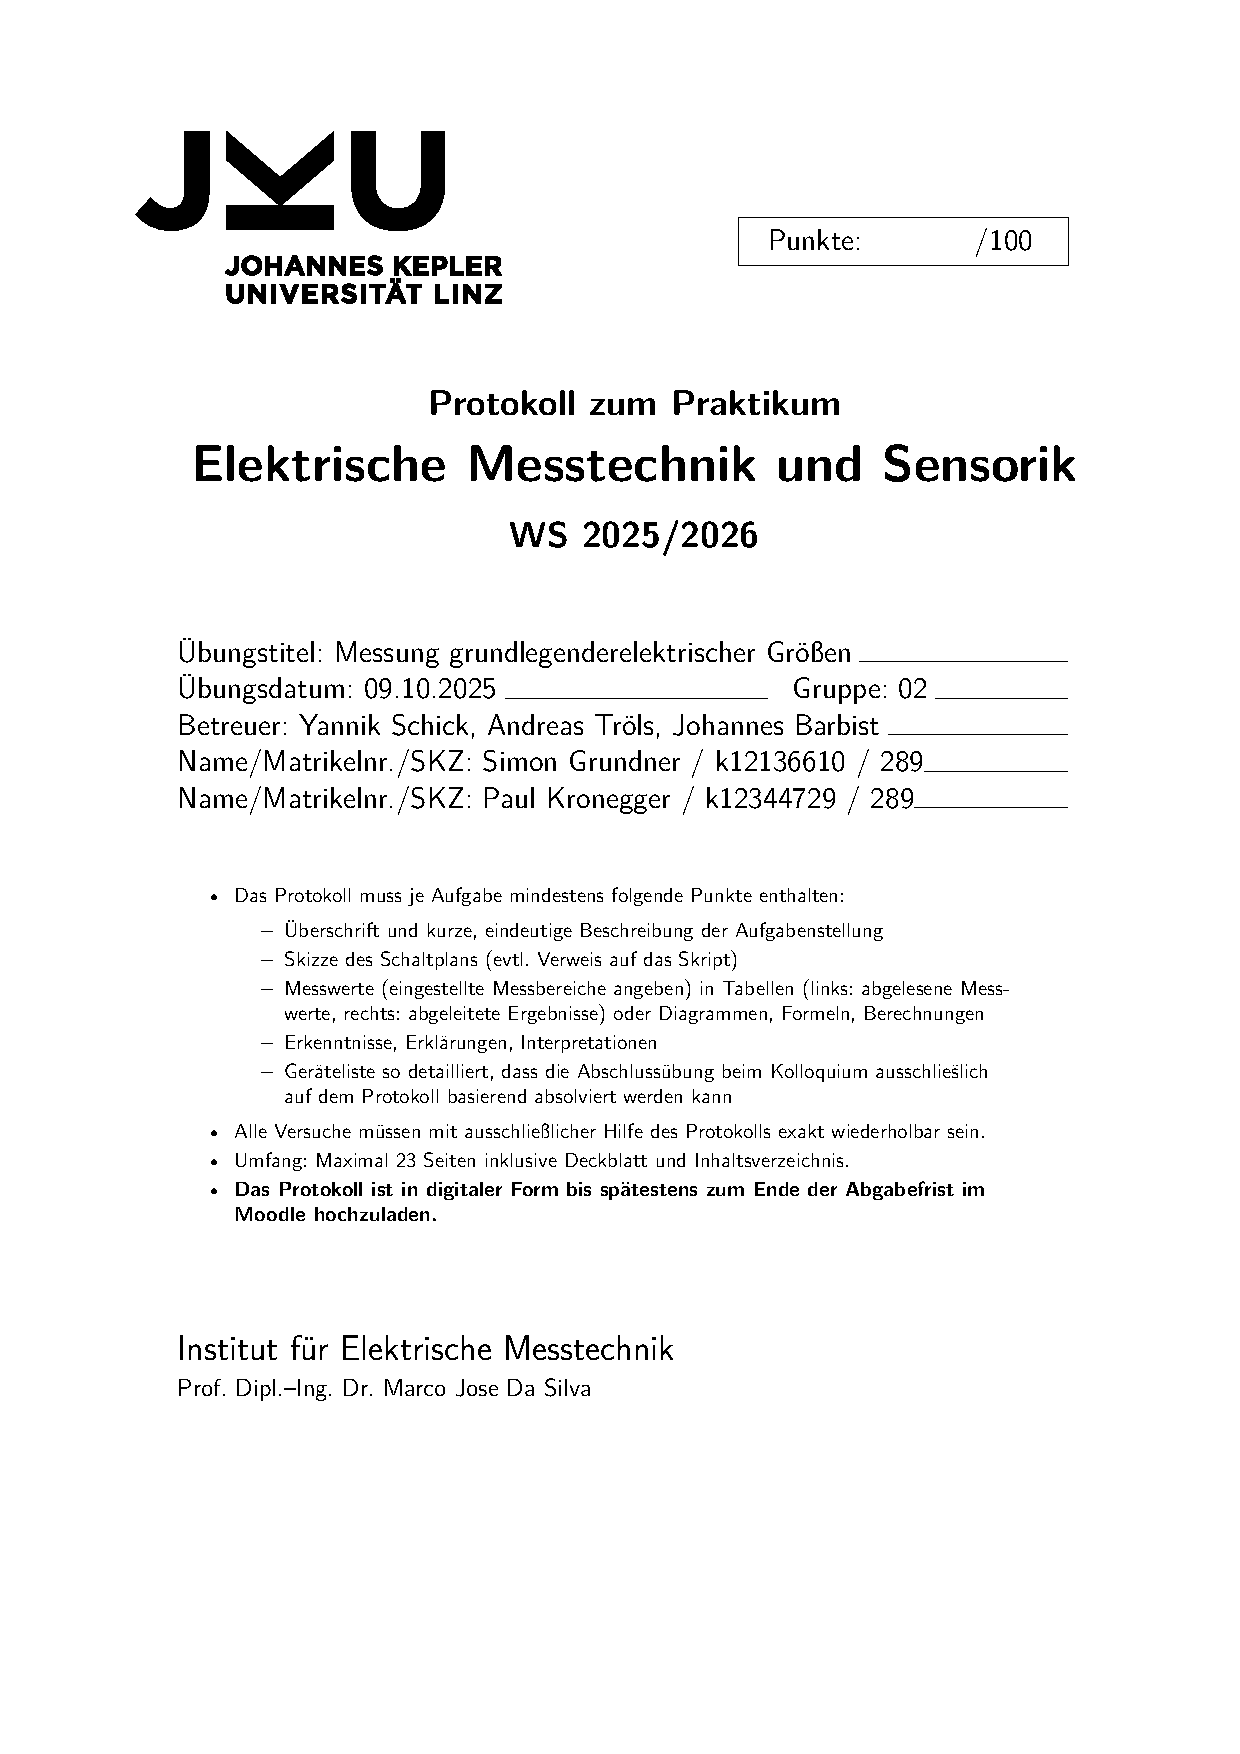
\includepdf{coversheet/coversheet.pdf}
\tableofcontents

\section{Geräteliste}\label{sec:geraeteliste}

\begin{table}[h]
    \centering
    \caption{Geräteliste}\label{tab:geraeteliste}
    \begin{tabularx}{\columnwidth}{cXXX}
        Pos & \textbf{Gerätebezeichnung} & \textbf{Modell} & \textbf{Anmerkungen}\\ \midrule
        1 & Multimeter & METEX M-4600 \\
        2 & Multimeter & METEX M-4630B \\
        3 & Multimeter & Fluke \\
        4 & Osilloskop & TDS2014C & \\
        5 & Netzteil & Hameg HM8040-2\\
        6 & Funktionsgenerator & 
    \end{tabularx}
\end{table}

\newpage
\section{Messung grundlegender elektrischer Größen}\label{sec:01}

\subsection{Widerstandsmessung I: Einzelmessung}\label{sec:01-1}

\begin{highlightblock}[Widerstand mit nur einer Messung bestimmen]
Ohmscher Leistungswiderstand, $R=\SI{68}{\ohm}, P_{\max}=\SI{50}{\watt}$
\begin{enumerate}[label=\textbf{\alph*:}, ref=\alph*]
    \item Strom oder Spannungsrichtig messen?\label{itm:P1-1}
    \item Passende Spannung wählen.\label{itm:P1-2}
    \item Kontrollieren, ob der systematische Fehler vernachlässigbar ist.\label{itm:P1-3}
    \item Garantiefehlergrenzen abschätzen.\label{itm:P1-4}
    \item Messung durchführen.\label{itm:P1-5}
\end{enumerate}
\end{highlightblock}\medskip

\marginref{\ref{itm:P1-1}}
Da der Widerstand sehr klein ist, wird für dessen Ermittlung eine
spannungsrichtige U-I-Messung durchgeführt
\cite[S.~183]{SchrüferElmar2022EM:M}.

\marginref{\ref{itm:P1-2}}
Um eine passende Spannung zu wählen, werden erst die Messbereiche der Geräte
abgeschätzt. Relevante Daten der verwendeten Messgeräte (Tabelle
\ref{tab:geraeteliste}; Pos 1, 2) sind die $\SI{100}{\milli\volt}$ über den Amperemeter shunt
und der Innenwiderstand des Voltmeters über alle Messbereiche $R_{iV} =
\SI{10}{\mega\ohm}$.

\begin{wrapfigure}[7]{r}{5cm}
\vspace{-20pt}\raggedleft
\captionsetup{justification=raggedleft, singlelinecheck=false, margin=10pt}
\begin{circuitikz}[scale=0.85, transform shape]
    \draw (0,0) to[voltage source, v<=$U$] (0,3) 
        to[ameter, i=$I_A$] (3,3) coordinate (k1)
        to[vmeter, v=$U_V$, i>^=$I_V$, *-*] (3,0) coordinate (k2) -- (0,0);
    \draw (k1) -- ++(1,0) to[R, l=$R$, i>^=$I_R$] ++(0,-3) -- (k2);
\end{circuitikz}
\caption{Spannungsrichtige\\U-I-Messung}\label{fig:u-i-spannungsrichtig}
\end{wrapfigure}

Daraus ergeben sich folgende Abschätzungen für den Messbereich in abhängigkeit der gewählten Spannung:

\begin{itemize}
    \item $U_V \sim U - \SI{200}{\milli\volt}$
    \item $I_A \sim (U - \SI{200}{\milli\volt}) \left(\dfrac{1}{R} + \dfrac{1}{R_{iV}}\right)$
\end{itemize}

Sei die gewählte Spannung $U=\SI{5}{\volt}$, so ergibt sich:

\begin{itemize}
    \item $U_V \sim \SI{4.8}{\volt} \implies \text{MB:}~\SI{20}{\volt}$
    \item $I_A \sim \SI{71}{\milli\ampere} \implies \text{MB:}~\SI{200}{\milli\ampere}$
\end{itemize}

\marginref{\ref{itm:P1-3}}
Aus der Schaltung~\ref{fig:u-i-spannungsrichtig} ergibt sich folgende
Gleichung für den gemessenen Widerstand:

\begin{equation}
R = \frac{U_V}{I_R} = \frac{U_V}{I_A-I_V} = \frac{U_V}{I_A-U_V/R_{iV}}
\label{eq:r-spannungsrichtig}
\end{equation}

Der systematische Fehler in der Strommessung wird hierbei durch den
Innenwiderstand des Voltmeters verursacht. Da aber aus $R \ll R_{iV}$ folgt,
dass $I_A \approx I_R$, ist der Fehler sehr gering, kann aber trotzdem
korrigiert werden, sofern $R_{iV}$ bekannt ist.

\marginref{\ref{itm:P1-4}}
Die Garantiefehlergrenzen der Messgeräte (Tabelle~\ref{tab:geraeteliste}; Pos 1, 2) sind für die gewählten Messbereiche:
\begin{itemize}
    \item Voltmeter: $u_{U_V} = \pm(\SI{0.05}{\percent} + 3 \text{ Digits})
        = \pm(\SI{0.05}{\percent} \cdot \SI{20}{\volt} + 3 \cdot \SI{0.001}{\volt})
        = \pm \SI{0.013}{\volt}$
    \item Amperemeter: $u_{I_A} = \pm(\SI{0.3}{\percent} + 3 \text{ Digits})
        = \pm(\SI{0.3}{\percent} \cdot \SI{200}{\milli\ampere} + 3 \cdot \SI{0.01}{\milli\ampere})
        = \pm \SI{0.63}{\milli\ampere}$
\end{itemize}

\newpage
\begin{wrapfigure}[13]{r}{5cm}
    \vspace{-12pt}\centering
    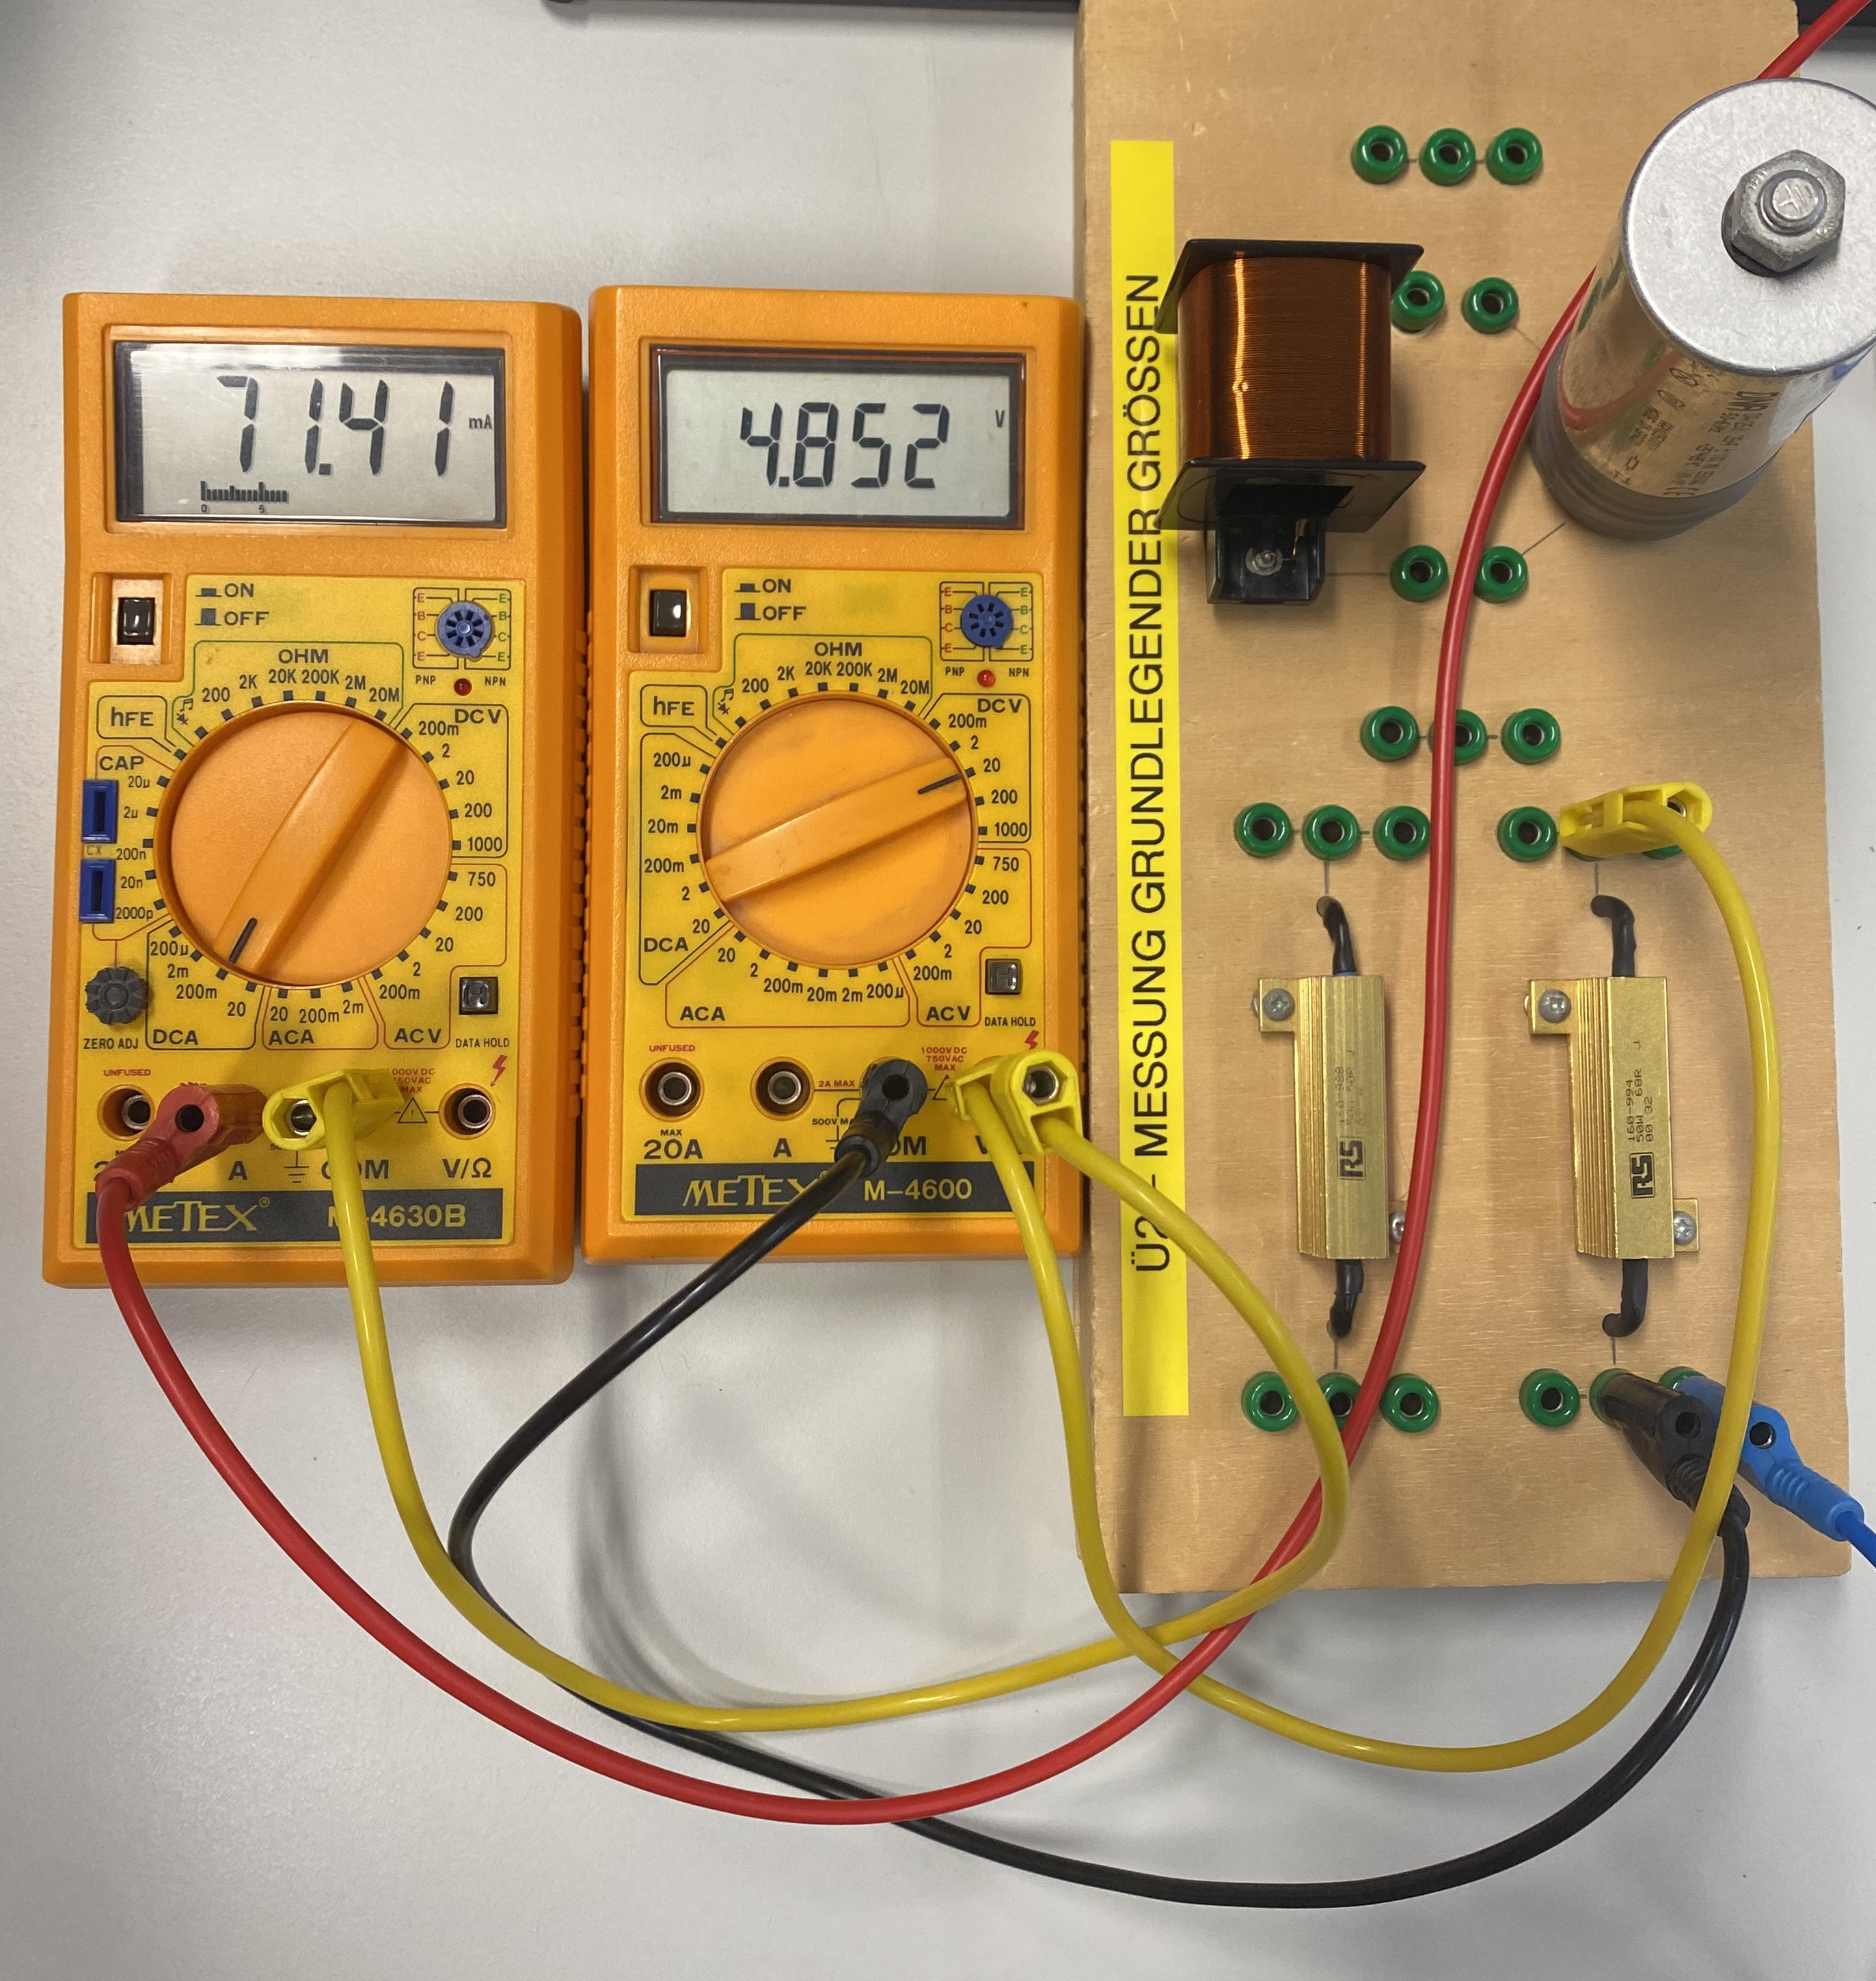
\includegraphics[width=5cm]{images/11_Aufbau.JPEG}
    \caption{Aufbau der Messung}\label{fig:11_aufbau}
\end{wrapfigure}

\marginref{\ref{itm:P1-5}}
Durchführung der Messung liefert die Messwerte für Strom und Spannung.
Anschließend wird der Widerstand mit Gleichung \ref{eq:r-spannungsrichtig} unter Anwendung der
Fehlerfortpflanzung~\cite[Gl.~1.80]{SchrüferElmar2022EM:M} berechnet.

\begin{itemize}
    \item $U_V = \SI{4.852}{\volt} \pm \SI{0.013}{\volt}$
    \item $I_A = \SI{71.41}{\milli\ampere} \pm \SI{0.63}{\milli\ampere}$ 
    \item $R = \SI{67.9}{\ohm} \pm \SI{0.6}{\ohm}$
\end{itemize}

Berechnung der Unsicherheit des Widerstandswertes:
\[
    u_R = \sqrt{{\left(\frac{\partial R}{\partial U}u_{U_V}\right)}^2 + {\left(\frac{\partial R}{\partial I}u_{I_A}\right)}^2} = \SI{0.6265}{\ohm}
\]
mit
\[
    \frac{\partial R}{\partial U}\Big|_{U=U_V} = \frac{I_A R_{iV}^2}{{(-I_A R_{iV} + U_V)}^2} =  \SI{14.00}{\ohm\per\volt}
\]
und
\[
    \frac{\partial R}{\partial I}\Big|_{I=I_A} = -\frac{U_{V}}{{(I_A - U_V/R_{iV})}^2} = -951.5 \si{\ohm\per\ampere}
\]
\newpage
\subsection{Widerstandsmessung II: Statistische Auswertung}\label{sec:01-2}

\begin{highlightblock}[Wiederholte Messungen mit statistischen Abweichungen]
\begin{enumerate}[label=\textbf{\alph*:}, ref=\alph*]
	\item Statistisch unabhängige Messung:\label{itm:P2-1}
	\begin{itemize}
		\item Unterschiedliche Werte von Strom- / Spannungswerte + Messbereiche
		\item Messgeräte tauschen.
		\item Kabel ein- und ausstecken
	\end{itemize}
	\item Messreihe statistisch auswerten (Schätzwert des Mittelwertes $\bar{x}$ und Standardabweichung~$s$)
	\item Konfidenzintervalle für Vertrauensniveaus: $1-\alpha =\{68.26\%, 99.5\%\}$ 
	\item Diskussion des Einflusses der unterschiedlichen Spannungsniveaus.
\end{enumerate} 
\end{highlightblock}

\subsubsection{Verwendetes Material}

\begin{table}[h]
	\centering
	\caption{Verwendetes Material}
	\begin{tabularx}{\textwidth}{XXX}
		\textbf{Material} & \textbf{Verwendung} & \textbf{Anmerkungen}\\ \midrule
		&  &  \\
		&  &  \\
		&  &  \\
	\end{tabularx}	
\end{table}

\subsubsection{Versuchsaufbau}

\marginref{\ref{itm:P2-1}}
Hier wurde der gleiche Versuchsaufbau wie in Abschnitt~\ref{sec:01-1} verwendet und folgende Messwerte Aufgenommen:

\begin{table}[h]
	\centering
	\caption{Messwerte Widerstandsmessung II}\label{tab:01-2-values}
	\pgfplotstabletypeset[
		col sep=comma,
		header=true,
		every head row/.style={after row=\midrule},
		begin table={\begin{tabularx}{\textwidth}},
		end table={\end{tabularx}},
		columns/desc/.style={column name={Bemerkung}, column type=|X, string type},
		columns/Nr/.style={column name={Nr}, column type=c},
		columns/U/.style={column name={$U / \si{\volt}$}, column type=c, precision=2, fixed},
		columns/UV/.style={column name={$U_V / \si{\volt}$}, column type=c, precision=2, fixed},
		columns/IA/.style={column name={$I_A / \si{\milli\ampere}$}, column type=c, precision=3, fixed},
		columns/R/.style={column name={$R / \si{\ohm}$}, column type=c, precision=2, fixed},
	]{../data/12_Values.csv}
\end{table}

\reversemarginpar\marginnote{\textbf{(\ref{itm:P1-2})}}[5pt]
Die Berechnung des Mittelwertes ($\bar{x}$) und der Standardabweichung~$s$~\cite[S.~7]{EMTPraktikum2025}:
\begin{align}
	& \bar{x} = \frac{1}{n} \sum_{i=1}^{n} x_i = \SI{67.94}{\ohm} \\
	& s = \sqrt{\frac{1}{n-1} \sum_{i=1}^n {(x_i - \bar{x})}^2} = \SI{0.08451}{\ohm} \approx \SI{0.08}{\ohm}
\end{align}

\reversemarginpar\marginnote{\textbf{(\ref{itm:P1-3})}}[5pt]
Das erweiterte Unsicherheitsintervall berechnet sich nach~\cite[S.~10, Tabelle~1.1]{EMTPraktikum2025} zu
\[
	u_{z} = t_{0} \frac{s}{\sqrt{n}} \, .
\]

Für $n=5$ ergibt sich:

\begin{itemize}
	\item 68,26\% Vertrauensniveau ($t_{0}/\sqrt{n} = 0.51$):
		\[
			u_{z} = 0.51 \cdot \SI{0.08}{\ohm} \approx \SI{0.041}{\ohm},
		\]
		also das Konfidenzintervall
		\[
			\bar{x} \pm u_{z} = (67.94 \pm 0.04) \, \si{\ohm}.
		\]

	\item 99,5\% Vertrauensniveau ($t_{0}/\sqrt{n} = 2.50$):
		\[
			u_{z} = 2.50 \cdot \SI{0.08}{\ohm} \approx \SI{0.175}{\ohm},
		\]
		also das Konfidenzintervall
		\[
			\bar{x} \pm u_{z} = (67.94 \pm 0.18) \, \si{\ohm}.
		\]
\end{itemize}

\reversemarginpar\marginnote{\textbf{(\ref{itm:P1-4})}}[5pt]
Einflusses der unterschiedlichen Spannungsniveaus:

Am Anfang des Strommessbereichs ist der relative Fehler am kleinsten (vgl. Messung~3).
Dies entspricht den Herstellerangaben zum Digitalmultimeter METEX~4600
(vgl. \cite[S.~143]{EMTPraktikum2025}), wonach der Fehler als Prozentwert des Anzeigewerts
angegeben wird. Bei kleinen Strömen (niedriges Spannungsniveau) ergibt sich daher die
geringste Abweichung, während diese bei höheren Spannungsniveaus zunimmt.


\newpage
\subsection{Widerstandsmessung III: Glühfaden}\label{sec:01-3}

\begin{highlightblock}[Temperatur eines Glühfadens]
Temperatur bei $U=\{40, 80, 120, 160, 200, 240\}$ Volt
\begin{enumerate}[label=\textbf{\alph*:}, ref=\alph*]
    \item R-Messung $R_\mathrm{kalt}$ des Glühfadens bei Umgebungstemperatur mit Ohmmeter\label{itm:P3-1}
    \item T-Messung der Raumtemperatur mit Thermometer.\label{itm:P3-2}
    \item U-I-Messung $R_\mathrm{heiss}$ des Glühfadens bei Betriebstemperatur mit den obrigen Spannungen.\label{itm:P3-3}
    \item Berechnung von $R(\theta_0)$ für $\theta_0=\SI{20}{\celsius}$.\label{itm:P3-4}
    \item Berechnung der Glühfadentemperatur bei bei den obrigen Spannungen aus $R_\mathrm{heiss}$.\label{itm:P3-5}
\end{enumerate}
\end{highlightblock}\medskip

\marginref{\ref{itm:P3-1},~\ref{itm:P3-2}}
Messung wie oben beschreiben ergibt $R_\mathrm{kalt} = \SI{30.9}{\ohm}$ und
$\theta_\mathrm{RT} = \SI{24.1}{\celsius}$.

\marginref{\ref{itm:P3-3}}

\begin{wrapfigure}[8]{r}{7cm}
    \vspace{-20pt}
    \centering
    \begin{circuitikz}[american inductors]
        \ctikzset{inductors/coils=6}
        \draw (0,0) coordinate (GND) to [sV] ++(0,2) coordinate (V1) -- ++(1,0) to[L] ++(0,-2) -- (GND);
        \draw (2,0) to[vL, name=L2] ++(0,2);
        \draw (L2.wiper) -- (L2.wiper |- V1)
            to[ameter, i=$I_A$] ++(2,0) coordinate (k1) 
            to[vmeter, v=$U_V$, *-*] (k1 |- GND) -- (2,0);
        \draw (k1) -- ++(1,0) to[lamp, l=$R_\mathrm{W}$, i>^=$I_R$] ++(0,-2) -- (k1 |- GND);
    \end{circuitikz}
    \caption{Aufbau der Messung}\label{fig:13-aufbau}
\end{wrapfigure}

Mit einem Variablen Trafo wurden die verschiedenen Spannungen eingestellt. Die
Schaltung wurde wie folgt aufgebaut: Die U-I-Messung wird wieder aufgrund des
niederohmigen Glühfadens mit einer Spannungsrichtigen Schaltung durchgeführt.
Der Widerstand ergibt sich somit wieder aus \autoref{eq:r-spannungsrichtig}.
Vor der Messung wird der erste Messbereich der Messgeräte für den
Kaltwiderstand wie in \autoref{sec:01-1} \autoref{itm:P1-2} abgeschätzt. Beim
ersten einschalten wird der höchste Strom erwartet, da der Glühdraht ein
Kaltleiter ist ($\alpha, \beta > 0$).

\begin{itemize}
    \item Voltmeter (M-4600): $U_V \sim \SI{40}{\volt}\implies$ MB: $\SI{200}{\volt}$
    \item Amperemeter (M-4630B): $I_A \sim \SI{1.3}{\ampere}\implies$ MB: $\SI{20}{\ampere}$
\end{itemize}

Sobald sich der Glühfaden erwärmt reduziert sich der Strom und der Messbereich
kann bei Bedarf angepasst werden. Die Messergebnisse (Effektivwerte) und der
daraus resultierende Widerstand sind in \autoref{tab:13-values} dargestellt.

\begin{table}[h]
    \centering
    \caption{Messergebnisse der Glühfadenmessung}\label{tab:13-values}
    \pgfplotstabletypeset[
        col sep=comma,
        header=true,
        every head row/.style={after row=\midrule},
        begin table={\begin{tabularx}{\textwidth}},
        end table={\end{tabularx}},
        columns/U/.style={column name={$U / \si{\volt}$}, column type=Y, precision=2, fixed},
        columns/UV/.style={column name={$U_V / \si{\volt}$}, column type=Y|, precision=2, fixed},
        columns/IA/.style={column name={$I_A / \si{\milli\ampere}$}, column type=Y, precision=3, fixed},
        columns/R/.style={column name={$R / \si{\ohm}$}, column type=Y, precision=2, fixed},
        columns/T/.style={column name={$T / \si{\celsius}$}, column type=Y, precision=2, fixed},
    ]{../data/13_Values.csv}
\end{table}

\marginref{\ref{itm:P3-4}}
Für die Temperaturabhängigkeit des Widerstands gilt die Näherung:

\begin{equation}
    R(\theta) = R(\theta_0) \cdot (1 + \alpha \cdot (\theta - \theta_0) + \beta \cdot (\theta - \theta_0)^2)
    \label{eq:gluehfaden}
\end{equation}

Für Wolfram sind die Temperaturkoeffizienten für $\theta_0=\SI{20}{\celsius}$:
$\alpha = \SI{4.1e-3}{\per\kelvin}$ und $\beta = \SI{1.0e-6}{\per\kelvin\squared}$.
Einsetzen der Messwerte aus \autoref{itm:P3-1} und \ref{itm:P3-2} in
\autoref{eq:gluehfaden} liefert:

\begin{equation*}
    R(\theta_0) = \frac{R_\mathrm{kalt}}{1 + \alpha \cdot (\theta_\mathrm{RT} - \theta_0) + \beta \cdot (\theta_\mathrm{RT} - \theta_0)^2} = \SI{30.39}{\ohm}
\end{equation*}

\marginref{\ref{itm:P3-5}}
Nun kann man die berechneten Widerstands Werte in die Linke Seite von \autoref{eq:gluehfaden}
einsetzen und mit einem Mathematik-Programm nach der Temperatur $\theta$ lösen. Die errechneten
Temperaturen wurden zu \autoref{tab:13-values} hinzugefügt.

\newpage
\subsection{Widerstandsmessung IV: Impedanzen}\label{sec:1-4}

\begin{highlightblock}[Messung Impedanzen, Drei-Voltmeter-Methode]
    Funktionsgenerator $20\mathrm{V_{SS}}$. $50\Omega$ Shuntwiderstand, 
    \begin{enumerate}[label=\textbf{\alph*:}, ref=\alph*]
        \item\label{itm:1-P4-1} Frequenz geeignet wählen.
        \item\label{itm:1-P4-2} Spannungsdreieck zeichnen. Daraus Betrag und Phase ablesen.
        \item\label{itm:1-P4-3} Ergebnis mit der Rechnung vergleichen.
    \end{enumerate}
\end{highlightblock}

\subsubsection{Verwendetes Material}

\begin{table}[h]
	\centering
	\caption{Verwendetes Material}
	\begin{tabularx}{\textwidth}{XXX}
		\textbf{Messgerät} & \textbf{Verwendung} & \textbf{Anmerkungen}\\ \midrule
		&  &  \\
		&  &  \\
		&  &  \\
	\end{tabularx}	
\end{table}

\subsubsection{Versuchsaufbau}

\marginref{\ref{itm:1-P4-1}}
Für die Frequenz wurde $f=\SI{1}{\kilo\hertz}$ gewählt. Bei dem
Frequenzgenerator war es nur möglich $\SI{10}{\volt}_{PP}$ einzustellen.
Anstelle von $R$ wurde ein Shuntwiderstand von $R=\SI{50}{\ohm}$ verwendet.
$Z$ ist hier entweder die zur verfügung gestellte Spule oder der Kondensator.

\begin{figure}[h]
    \centering
    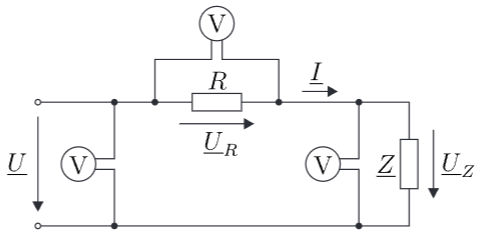
\includegraphics[width=7cm]{images/14_Aufbau.png}
    \caption{Aufbau der Messung}\label{fig:14-aufbau}
\end{figure}

\marginref{\ref{itm:1-P4-2}}

Für die drei Messgeräte ergeben sich folgende Einzelmesswerte:

\begin{table}[h]
    \caption{Messergebnisse der 3-Voltmeter-Methode}\label{tab:14-values}
    \begin{tabularx}{\textwidth}{XYYY}
        \textbf{Bauteil} & $U / \si{\volt}$ & $U_R / \si{\volt}$ & $U_Z / \si{\volt}$ \\ \midrule
        Kondensator & 3.45 & 3.367 & 0.315 \\
        Spule & 5.534 & 2,151 & 4.807
    \end{tabularx}
\end{table}

\newpage

Mit diesen Effektivwerten der Spannungen können nun die Spannungsdreiecke
mit Lineal und Zirkel konstruiert werden, oder wie hier in GeoGebra:

\begin{figure}[h]
\begin{minipage}[position]{0.48\textwidth}
    \centering
    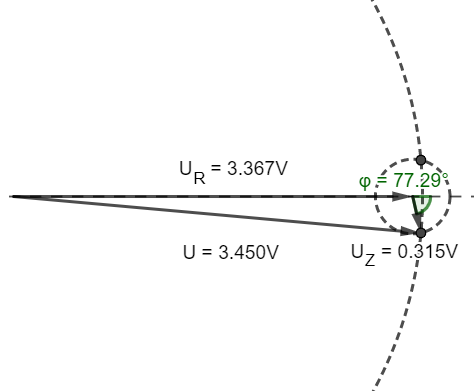
\includegraphics[height=4.5cm]{images/14_3-Voltmeter_C.png}
    \caption{Spannungsdreieck des Kondensators}
\end{minipage}\hfill
\begin{minipage}[position]{0.48\textwidth}
    \centering
    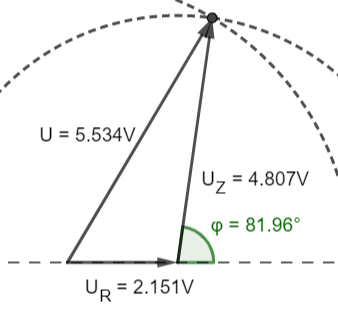
\includegraphics[height=4.5cm]{images/14_3-Voltmeter_L.png}
    \caption{Spannungsdreieck der Spule}
\end{minipage}
\end{figure}

Formeln für Betrag und Phase der Impedanz~\cite[S.~21]{EMTPraktikum2025}:

\[
    |Z| = \frac{U_C}{U_R/R} \qquad |\varphi_C| = \arccos\left(\frac{U^2-U_R^2-U_Z^2}{2U_Z U_R}\right)
\]

\begin{minipage}[t]{0.48\textwidth}

    Da bekannt ist, dass die gemessene impedanz Kapazitiv ist, ist das Vorzeichen des Winkels negativ.

    \[
        \begin{aligned}
            |Z_C| &= \frac{\SI{0.315}{\volt}}{\SI{3.367}{\volt}/\SI{50}{\ohm}} = \SI{4.678}{\ohm} \\
            \varphi_C & = \SI{-1.349}{\radian} = \SI{-77.3}{\degree}\\
        \end{aligned}
    \]

\end{minipage}\hfill
\begin{minipage}[t]{0.48\textwidth}

    Da bekannt ist, dass die gemessene impedanz Induktiv ist, ist das Vorzeichen des Winkels positiv.

    \[
        \begin{aligned}
            |Z_L| &= \frac{\SI{4.807}{\volt}}{\SI{2.151}{\volt}/\SI{50}{\ohm}} = \SI{111.7}{\ohm} \\
            \varphi_L &= \SI{1.431}{\radian} = \SI{82.0}{\degree} \\
        \end{aligned}
    \]

\end{minipage}

\marginref{\ref{itm:1-P4-3}}
Um die einzelnen Werte der Komponenten zu erhalten, werden die Impedanzen in in
Real- und Imaginärteil zerlegt: $Z = R + \jmath X$

\begin{minipage}[position]{0.48\textwidth}
    \[
        \begin{aligned}
            R_C &= |Z_C| \cdot \cos(\varphi_C) = \SI{1.029}{\ohm} \\
            \jmath X_C &= \jmath |Z_C| \cdot \sin(\varphi_C) = -\jmath\SI{4.536}{\ohm}
        \end{aligned}
    \]
\end{minipage}\hfill
\begin{minipage}[position]{0.48\textwidth}
    \[
        \begin{aligned}
            R_L &= |Z_L| \cdot \cos(\varphi_L) = \SI{15.62}{\ohm} \\
            \jmath X_L &= \jmath |Z_L| \cdot \sin(\varphi_L) = \jmath\SI{111.7}{\ohm}
        \end{aligned}
    \]
\end{minipage}

\medskip
Umrechnen in Kapazität und Induktivität und den äquivalenten Serienwiderstand (ESR), jeweils bei $f=\SI{1}{\kilo\hertz}$:

\begin{minipage}[position]{0.48\textwidth}
    \[
        \begin{aligned}
            C &= -\frac{1}{2\pi f X_C} = \SI{35.1}{\micro\farad} \\
            R_{\mathrm{ESR}} &= R_C = \SI{1.029}{\ohm}
        \end{aligned}
    \]
\end{minipage}\hfill
\begin{minipage}[position]{0.48\textwidth}
    \[
        \begin{aligned}
            L &= \frac{X_L}{2\pi f} = \SI{17.8}{\milli\henry} \\
            R_{\mathrm{ESR}} &= R_L = \SI{15.62}{\ohm}
        \end{aligned}
    \]
\end{minipage}

\subsubsection{Erkenntnisse}

Hier wurde unglücklicherweise der Vorwiderstand von $R_V=\SI{68}{\ohm}$ bei der
Kondensatormessung nicht berücksichtigt, was zu einem schlechtem Verhältnis von
$U_Z$ zu $U_R$ führt. Dadurch wirken sich Messfehler bei den gemessenen
Spannungen stärker auf das Ergebnis aus. Weiters hätte die Frequenz beider
Messungen angepasst werden können, sodass bei den Impedanzen und dem
Shunt-Widerstand etwa die selbe Spannung abfällt, um den Messbereich weiter zu
verbessern.

% Beispielrechnung einfügen
\section{Oszilloskop}\label{sec:2}
\subsection{AC-DC Kopplung}\label{sec:2-1}

\begin{highlightblock}[Darstellung eines Rechtecksignals mit AC-DC Kopplung]
	Hier wird die AC- und DC-Kopplung des Oszilloskops verglichen, indem ein Rechtecksignal 
	auf zwei Kanäle mit den unterschiedlichen Kopplungsarten aufgeschalten wird.
	\begin{enumerate}[label=\textbf{\alph*:}, ref=\alph*, noitemsep]
		\item\label{itm:2-P1-1} Kanal 1 auf DC- und Kanal 2 auf AC-Kopplung einstellen.
		\item\label{itm:2-P1-2} Rechtecksignal mit $\SI{50}{\hertz}$ und $\SI{5}{\volt}_{PP}$ Amplitude ohne DC-offset aufschalten.
		\item\label{itm:2-P1-3} Kurvenformen vergleichen. Signale im Zeit- und Frequenzbereich analysieren.
	\end{enumerate}
	
\end{highlightblock}

\subsubsection{Verwendetes Material}

\begin{table}[h]
	\centering
	\caption{Verwendetes Material}
	\begin{tabularx}{\textwidth}{XXX}
		\textbf{Messgerät} & \textbf{Verwendung} & \textbf{Anmerkungen}\\ \midrule
		TDS2014C & Oszilloskop & $Z_E = \SI{1}{\mega\ohm}||\SI{20}{\pico\farad}$ \\
		Agilent 33250A & Funktionsgenerator &  \\
	\end{tabularx}	
\end{table}

\subsubsection{Versuchsaufbau}

\marginref{\ref{itm:2-P1-1},~\ref{itm:2-P1-2}}

Der Ausgang des Funktionsgenerators wird mit einem T-Glied Aufgeteilt und über
Koaxialkabeln mit beiden Kanälen des Oszilloskops verbunden.

\begin{figure}[h]
	\centering
	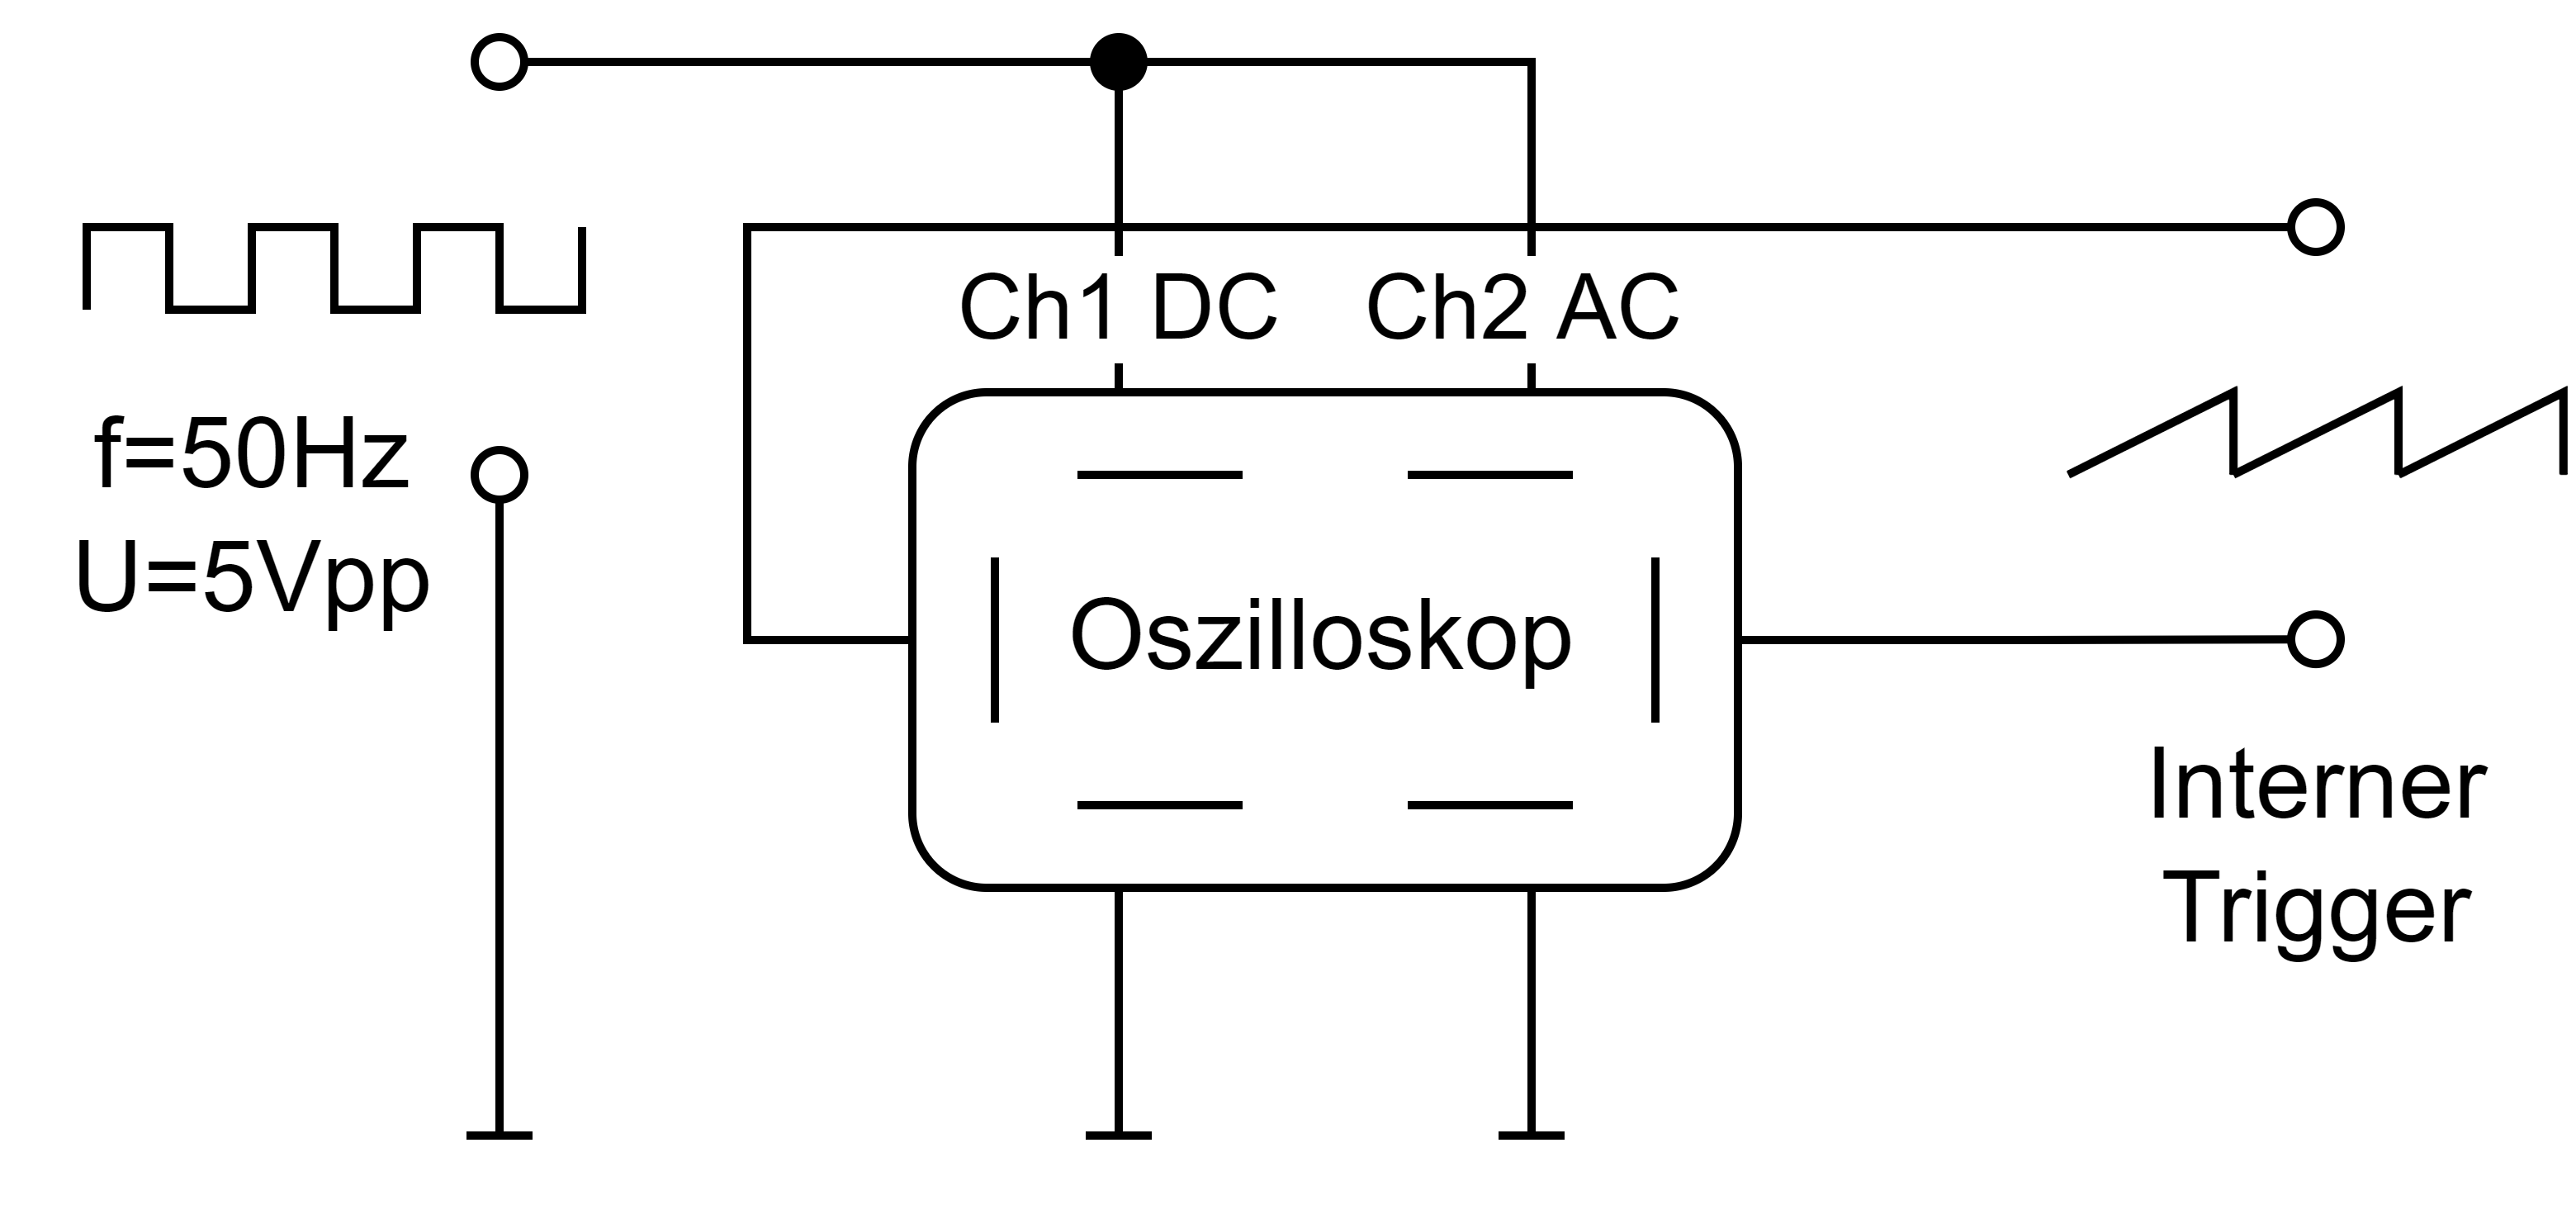
\includegraphics[width=7cm]{images/21_Aufbau.png}
	\caption{Schaltplan des Versuchsaufbaus}\label{fig:21-aufbau}
\end{figure}

Die Geräte werden folgdendermaßen konfiguriert:

\begin{minipage}[t]{.48\textwidth}
Einstellungen des Oszilloskops:

\begin{itemize}[noitemsep]
	\item Kanal 1 (DC): $\SI{2}{\volt}/\text{Div}$, $\SI{2.50}{\ms}/\text{Div}$
	\item Kanal 2 (AC): $\SI{2}{\volt}/\text{Div}$, $\SI{2.50}{\ms}/\text{Div}$
	\item Trigger: Kanal 1, falling edge
\end{itemize}
\end{minipage}\hfill
\begin{minipage}[t]{.48\textwidth}
Einstellungen des Funktionsgenerators:

\begin{itemize}[noitemsep]
	\item Frequenz: $\SI{50}{\hertz}$
	\item Amplitude: $\SI{5}{\volt}_{PP}$
	\item Wellenform: Rechteck
\end{itemize}
\end{minipage}

\newpage
Am Bildschirm des Oszilloskops sind nun die beiden Rechtecksignale zu sehen. 

\begin{figure}[h]
	\centering
	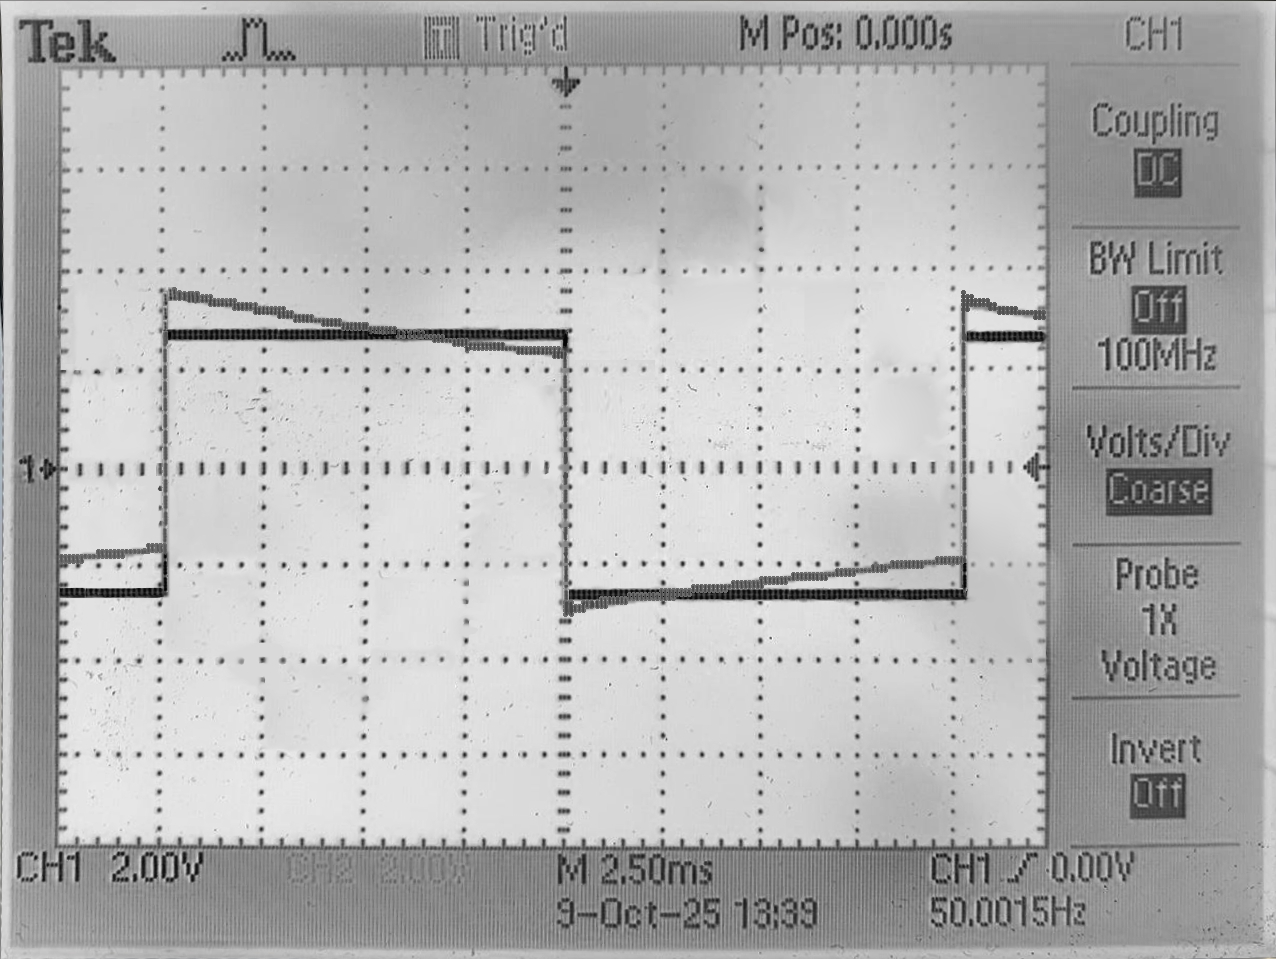
\includegraphics[width=5.5cm]{images/21_AC-DC-oszillogramm.jpg}
	\caption{Oszillogramm des Rechtecksignals beider Kanäle}
\end{figure}

\subsubsection{Erkenntnisse}

\marginref{\ref{itm:2-P1-3}}
Es ist zu erkennen, dass der Kanal mit DC Kopplung das ursprüngliche
Rechtecksignal übernimmt, während der Kanal mit AC Kopplung das Signal verformt.

\textbf{Im Zeitbereich} ist diese Verformung charakteristisch für die Entladekurve eines Kondensators,
welcher sich in Serie zur Messspitze befindet, um Gleichspannungsanteile zu blockieren.

\begin{wrapfigure}[7]{r}{7cm}
	\centering
	\vspace{-25pt}
	\begin{circuitikz}[scale=0.8, transform shape]
		\draw (0,0) node[anchor=east]{$U_\mathrm{E}$} to[C, l=$C_\mathrm{AC}$, o-*] ++(2,0) coordinate (k1)
			to[R=$R_\mathrm{E}$] ++(0,-2) node[rground] {};
		\draw (k1) -- ++(2,0) to[C=$C_\mathrm{E}$, color=lightgray] ++(0,-2) node[rground] {};
		\draw (k1) ++(2,0) to[short, *-o] ++(2,0) node[anchor=west]{$U_\mathrm{A}$}; 
	\end{circuitikz}
	\caption{Eingangsstufe eines AC-gekoppelten Kanals}
\end{wrapfigure}

Der Kondensator $C_\mathrm{AC}$ bildet zusammen mit der Eingangsimpedanz
$R_\mathrm{E}||C_\mathrm{E}$ des Oszilloskops einen Hochpass erster Ordnung. Die
Eingangsstufe des AC-gekoppelten Kanals kann somit durch folgende Schaltung
beschrieben werden. Die geringe Kapazität $C_\mathrm{E}$ des Oszilloskopeingangs
kann in diesem Frequenzbereich vernachlässigt werden.

\textbf{Im Frequenzbereich} belegt ein Periodisches Rechtecksignal alle ungeraden
Harmonischen seiner Grundfrequenz. Die Amplituden der Harmonischen nehmen mit
steigender Frequenz ab. Durch das gegenüberstellen mit der Übertragungsfunktion
des Hochpasses wird ersichtlich, dass die niederfrequenten Anteile des
Rechtecksignals gedämpft werden. Diese Dämpfung macht sich im Zeitbereich als
Verformung des Rechtecksignals bemerkbar.

\begin{figure}[h]
	\begin{minipage}[t]{.48\textwidth}
		\centering
		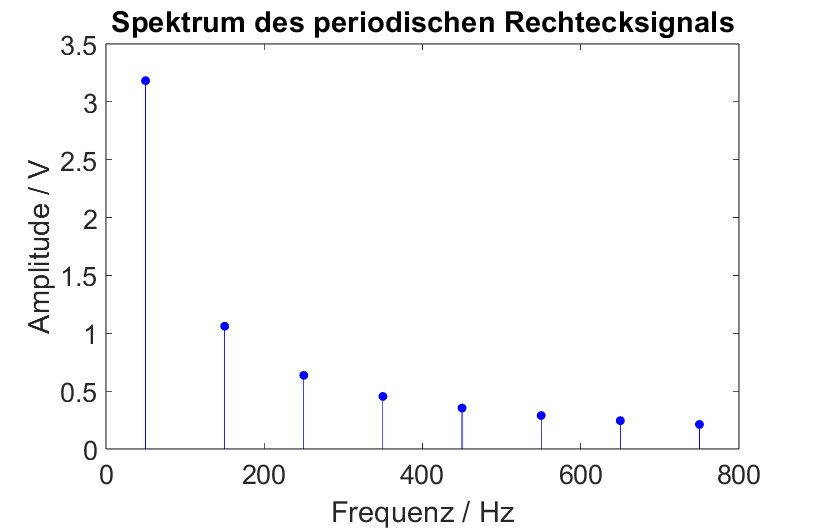
\includegraphics[height=4cm]{images/Spektrum-Squarewave.jpg}
		\caption{Spektrum eines Rechtecksignals}
	\end{minipage}\hfill
	\begin{minipage}[t]{.48\textwidth}
		\centering
		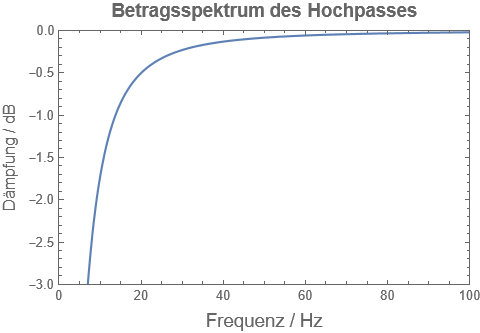
\includegraphics[height=4cm]{images/HochpassAbs.png}
		\caption{Betrag der Übertragungsfunktion des Hochpasses}
	\end{minipage}
\end{figure}
\newpage
\subsection{Grenzfrequenz des Hochpasses}\label{sec:2-2}

\begin{highlightblock}[Grenzfrequenz des Hochpasses der AC-Kopplung]
	Es soll ermittelt werden, welche Grenzfrequenz der Hochpass der AC-Kopplung des
	Oszilloskops aufweist. Hierzu gibt es zwei Methoden, die im Versuchsaufbau beschrieben
	werden. Im Anschluss kann die Kapazität des Koppelkondensators berechnet werden.
	\begin{enumerate}[label=\textbf{\alph*:}, ref=\alph*, noitemsep]
		\item\label{itm:2-P2-1} Methode A: Speisung mit einer Sinusspannung variabler Frequenz.
		\item\label{itm:2-P2-2} Methode B: Speisung mit einem niederfrequenten Rechtecksignal.
		\item\label{itm:2-P2-3} Berechnung der Kapazität $C_\mathrm{AC}$ des Koppelkondensators.
	\end{enumerate}
\end{highlightblock}

\subsubsection{Verwendetes Material}

\begin{table}[h]
	\centering
	\caption{Verwendetes Material}
	\begin{tabularx}{\textwidth}{XXX}
		\textbf{Messgerät} & \textbf{Verwendung} & \textbf{Anmerkungen}\\ \midrule
		TDS2014C & Oszilloskop & \\
		Agilent 33250A & Funktionsgenerator & \\
	\end{tabularx}	
\end{table}

\subsubsection{Versuchsaufbau}

\marginref{\ref{itm:2-P2-1}}

Bei der ersten Methode macht man sich zunutze, dass die Amplitude eines
Sinussignals bei der 3dB-Grenzfrequenz auf $\frac{1}{\sqrt{2}}$ des
ursprünglichen Wertes abgefallen ist. Am Funktionsgenerator wird eine
Sinusspannung mit $\SI{5}{\volt}_{PP}$ Amplitude und variabler Frequenz
eingestellt.

Sobald die Frequenz so weit erhöht wurde, dass die Amplitude auf
$\frac{1}{\sqrt{2}}\cdot\SI{5}{\volt}_{PP} \approx \SI{3.54}{\volt}_{PP}$
abgefallen ist, wird die Frequenz abgelesen. Diese entspricht der Grenzfrequenz
$f_g$ des Hochpasses. Wie man im \autoref{fig:21-3db-grenzfrequenz} sieht,
liegt die Grenzfrequenz bei $\SI{7}{\hertz}$.

\begin{figure}[h]
	\centering
	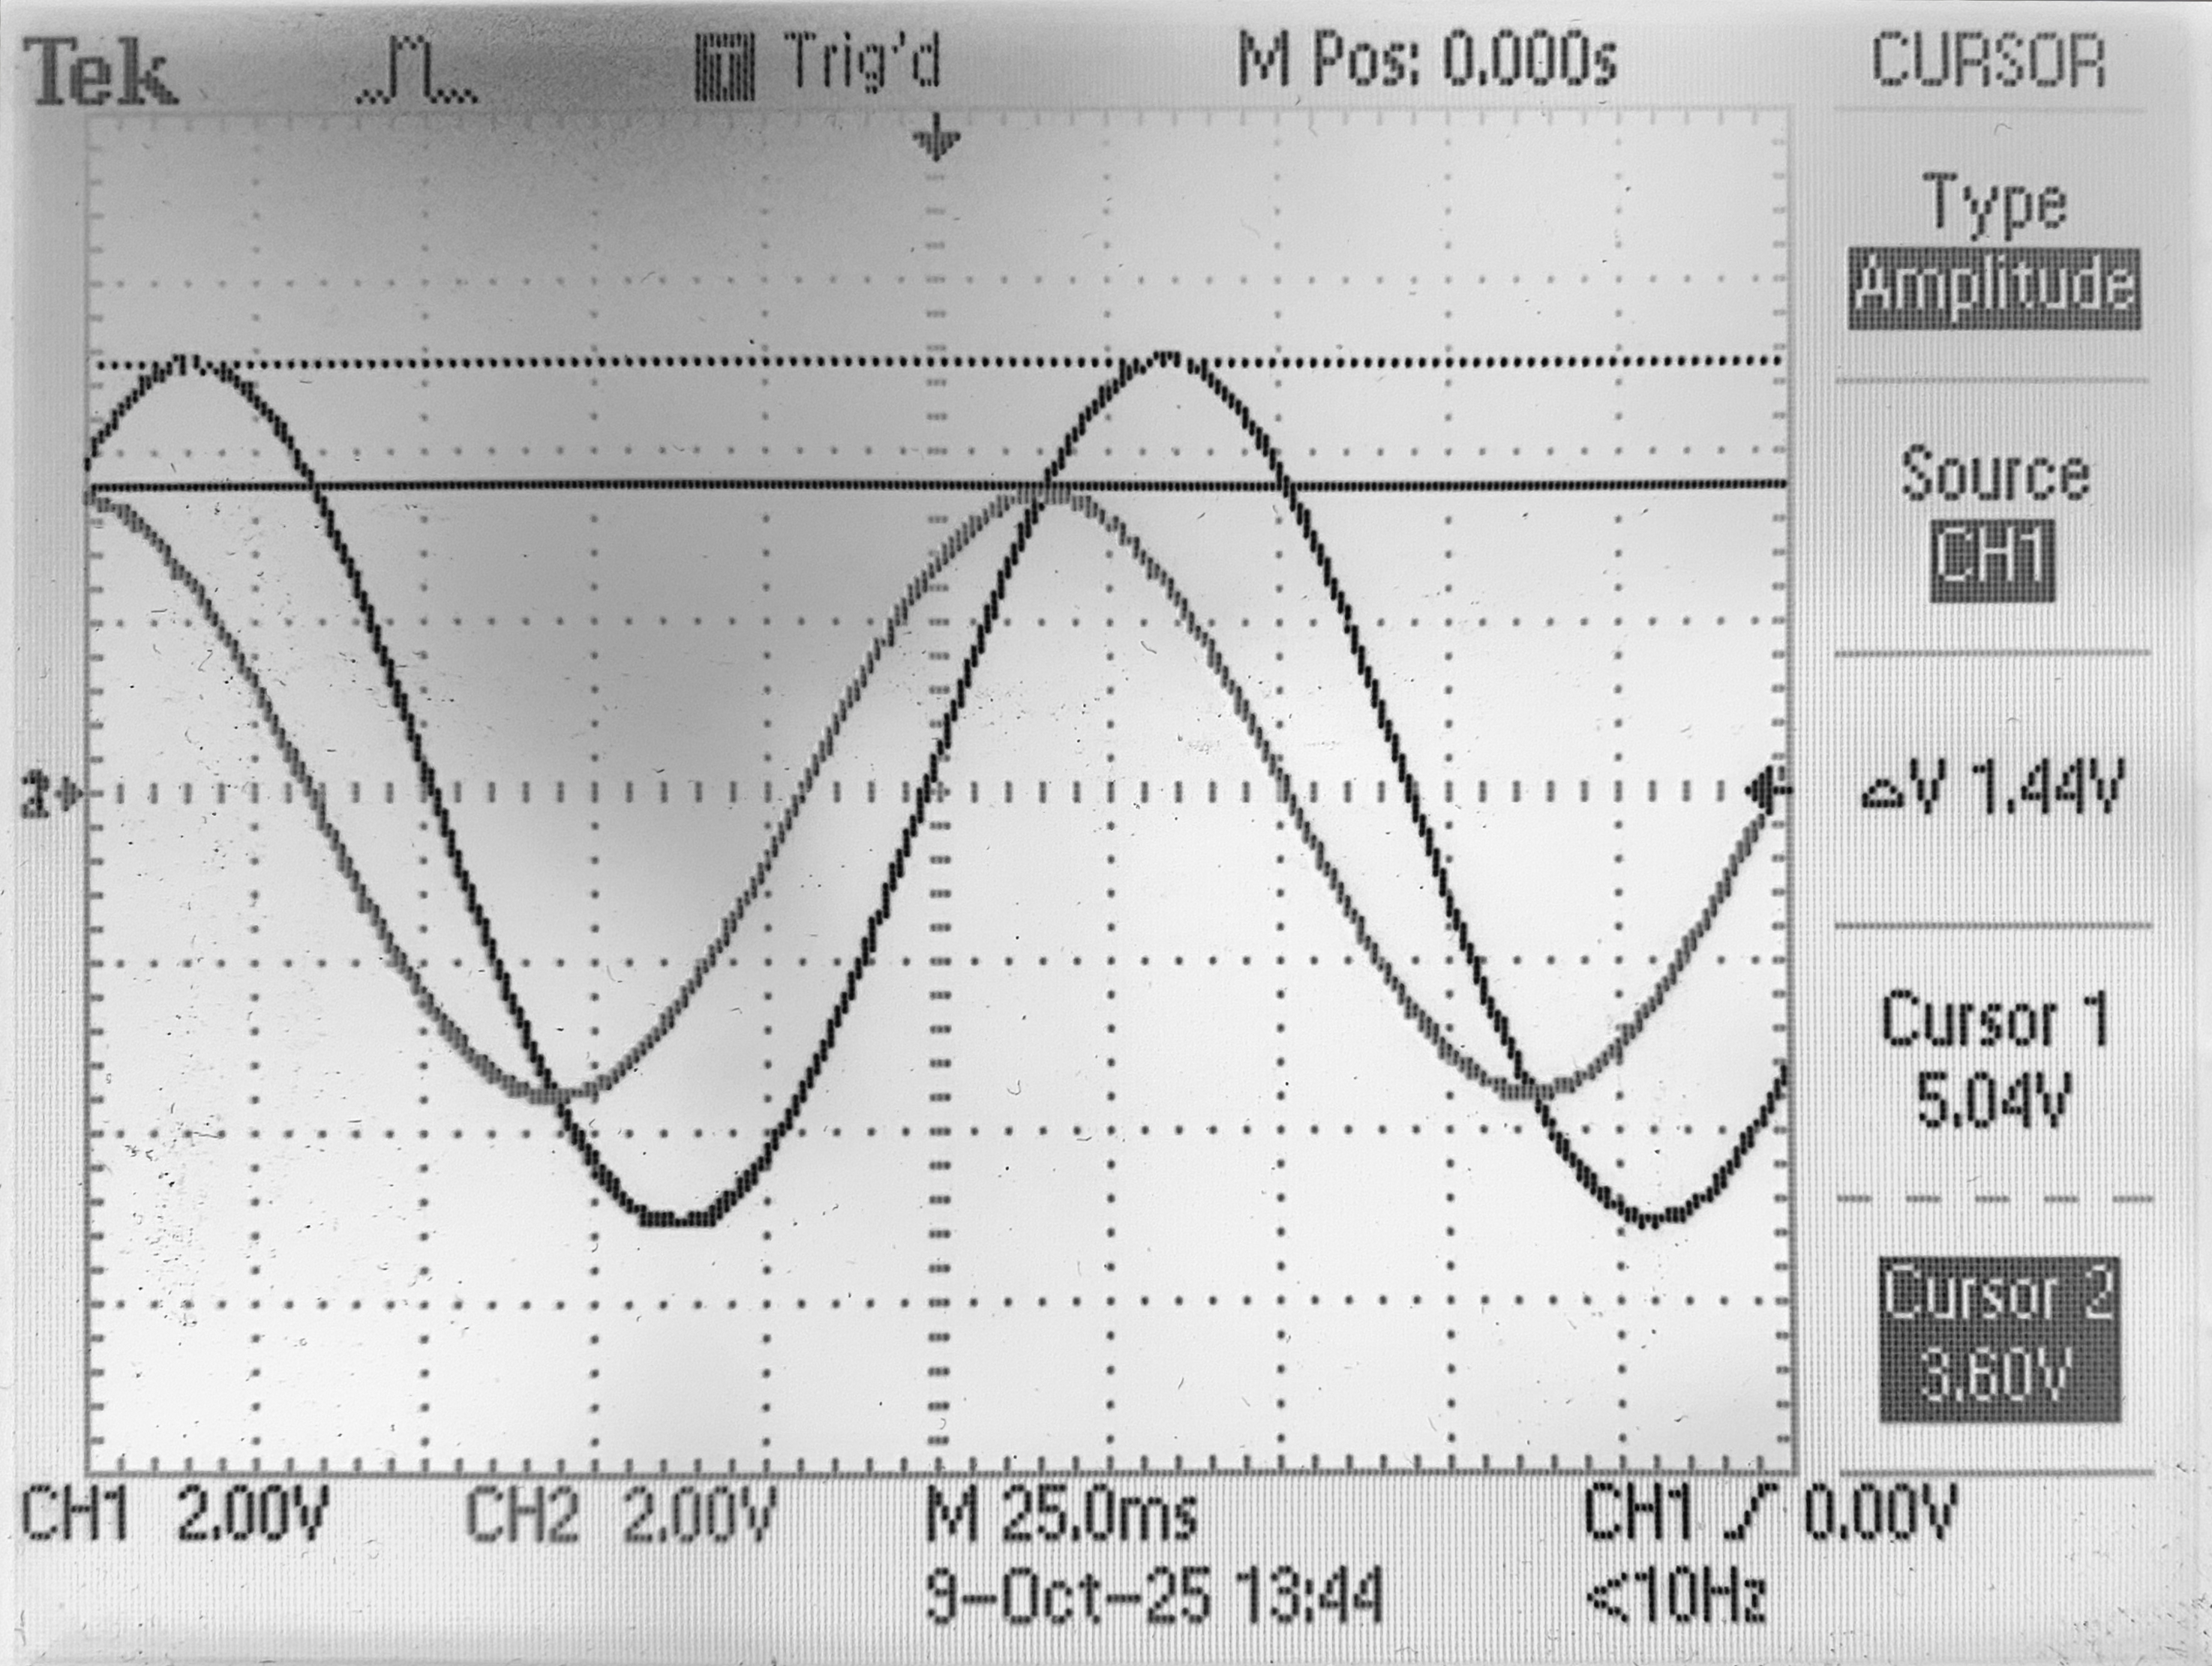
\includegraphics[width=7cm]{images/22_C-AC_Methode1.JPEG}
	\caption{Oszillogramm mit der 3dB Grenzfrequenz}
	\label{fig:21-3db-grenzfrequenz}
\end{figure}

\marginref{\ref{itm:2-P2-2}}

\begin{figure}[h]
	\centering
	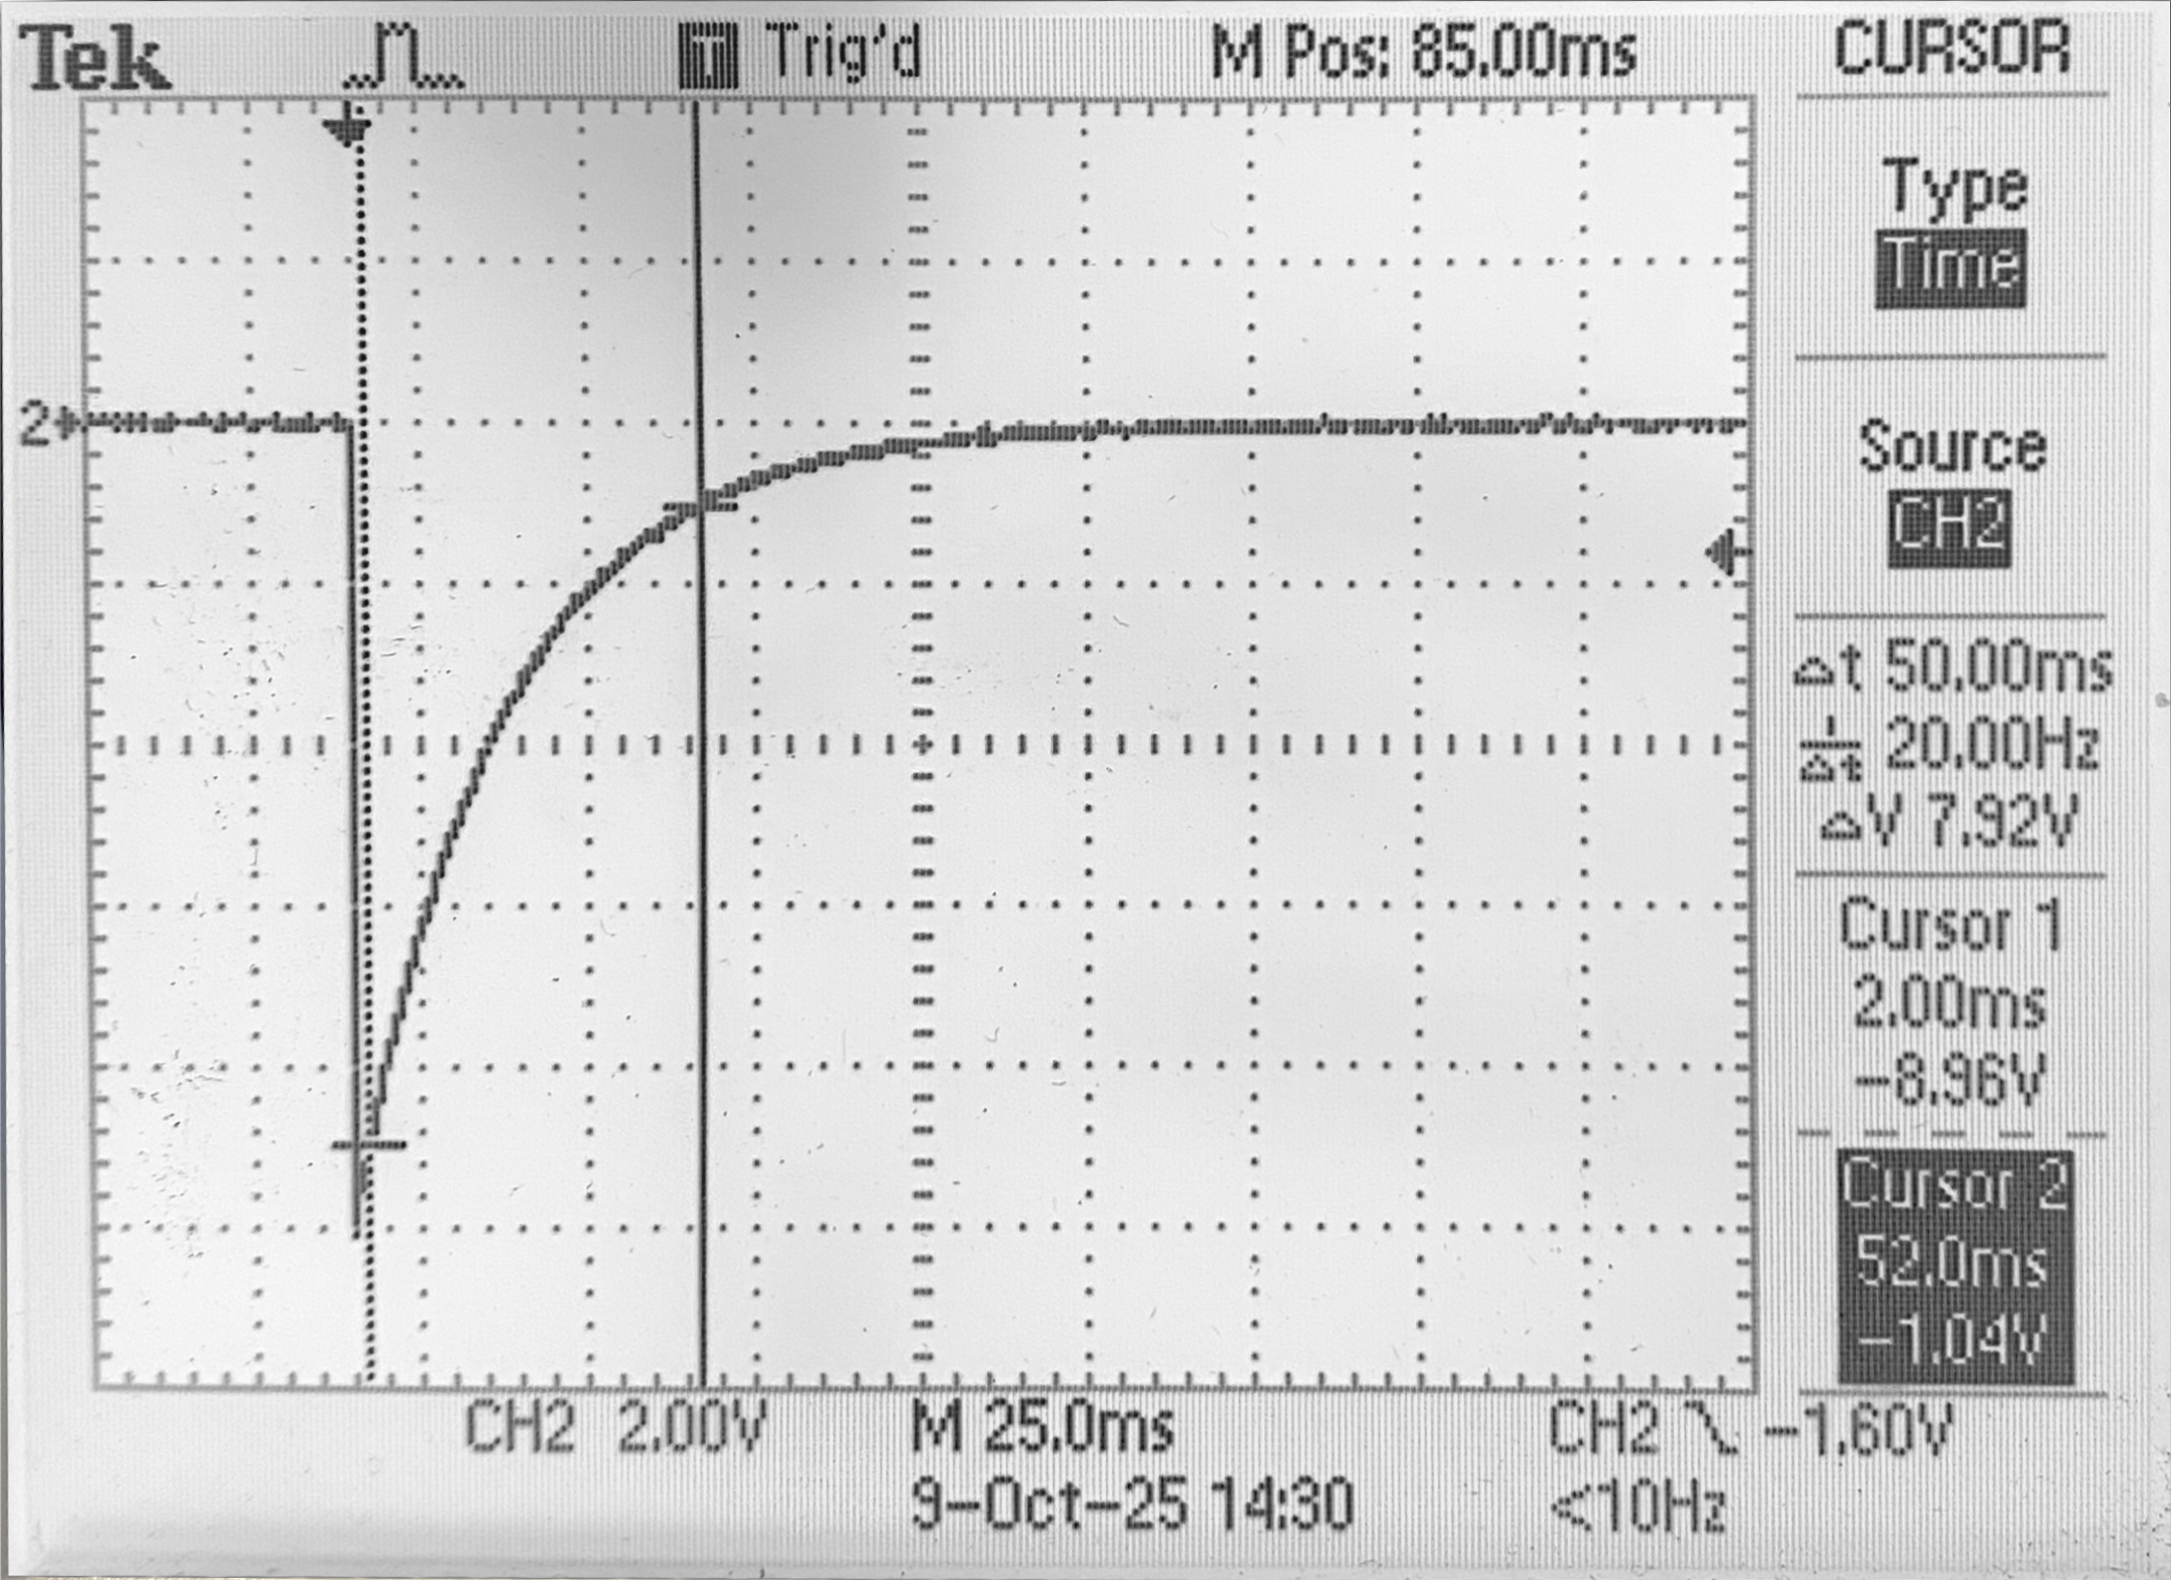
\includegraphics[width=7cm]{images/22_C-AC_Methode2.JPEG}
	\caption{Oszillogramm mit 10\%-90\% Anstiegszeit}
	\label{fig:21-10-90-anstiegszeit}
\end{figure}


\marginref{\ref{itm:2-P2-3}}

\subsubsection{Erkenntnisse}
\subsection{Eingangsimpedanz bei AC-Kopplung}\label{sec:2-3}

\begin{highlightblock}[Berechnung der Eingangsimpedanz bei AC-Kopplung]
	Rechnerische Ermittlung des Betrages der gesamten Eingangsimpedanz (\autoref{fig:impedanz-oszi-ac-kopplung}) des verwendeten
	Oszilloskops mit angeschlossenem Kabel und AC–Kopplung für eine Kabelkapazität von
	$C_K = \SI{100}{\pico\farad}$ und eine Frequenz von $f = \SI{1}{\mega\hertz}$.

\end{highlightblock}

\subsubsection{Verwendetes Material}

\begin{table}[h]
	\centering
	\caption{Verwendetes Material}
	\begin{tabularx}{\textwidth}{XXX}
		\textbf{Messgerät} & \textbf{Verwendung} & \textbf{Anmerkungen}                                \\ \midrule
		TDS2014C           & Oszilloskop         & $Z_E = \SI{1}{\mega\ohm}\,||\,\SI{20}{\pico\farad}$ \\
		Agilent 33250A     & Funktionsgenerator  &                                                     \\
	\end{tabularx}
\end{table}

\subsubsection{Berechnung}

\begin{wrapfigure}[6]{r}{0.4\textwidth}
	\vspace{-32pt}\centering
	\begin{circuitikz}[scale=1.1]
		\ctikzset{bipoles/length=1cm}
		\draw (0,2) to[open, v=$U_E$, o-o] (0,0);
		\draw (0,2)
			-- ++(1,0) coordinate (k1)
			to[C, l=$C_{AC}$] ++(2,0) coordinate (k2)
			-- ++(1,0)
			to[R, l=$R_E$] ++(0,-2)
			-- (0,0); 
		\draw (k1) to[C, l=$C_K$, *-*] ++(0,-2);
		\draw (k2) to[C, l=$C_E$, *-*] ++(0,-2);
	\end{circuitikz}
	\caption{Eingangsimpedanz des Oszilloskopes bei AC-Kopplung}\label{fig:impedanz-oszi-ac-kopplung}
\end{wrapfigure}

Zur Berechnung der Gesamt-Eingangsimpedanz $Z$ betrachtet man das Ersatzbild in
\autoref{fig:impedanz-oszi-ac-kopplung}. $C_{AC}$ ist der errechnete Wert aus
\autoref{sec:2-3} \autoref{itm:2-P2-3}
\begin{itemize}[noitemsep]
	\item $R_E =\SI{1}{\mega\ohm}$
	\item $C_E =\SI{20}{\pico\farad}, C_K=\SI{100}{\pico\farad}, C_{AC}=\SI{22.7}{\nano\farad}$
	\item $\omega =2\pi\cdot \SI{1}{\mega\hertz}$
\end{itemize}

Es ergibt sich für die Gesamteingangsimpedanz $Z$ der Ausdruck (wobei $\jmath X = 1/\jmath\omega C$):
\begin{align}
	Z &= \jmath X_K \parallel \bigl(\jmath X_{AC} + (\jmath X_{E} \parallel R_E)\bigr) \nonumber\\
	&= \frac{
		1 + \jmath\omega R_E\bigl(C_{E} + C_{AC}\bigr)
	}{
		\omega^2 R_E\bigl(-C_E C_K - C_{AC} C_K - C_E C_{AC}\bigr) +
		\jmath \omega\bigl(C_K + C_{AC}\bigr)
	}
\label{eq:eingangswiderstand_oszi}
\end{align}

Ergebnis für eingesetzte Bauteilwerte:
\[
Z = (1.76-\jmath 1326.48)\si{\ohm} 
  = \SI{1326.48}{\ohm} \angle \SI{-89.92}{\degree}
  \implies |Z| \approx \SI{1346.5}{\ohm}
\]

\subsubsection{Erkenntnisse}

Die Eingangsimpedanz befindet sich hier im Kiloohm Bereich. Für empfindliche
Messungen könnte das bereits eine zu hohe belastung sein, und das Ergebnis
würde verfälscht werden.



\subsection{Abgleich des Tastkopfes}\label{sec:2-4}

\begin{highlightblock}[Abgleich des Tastkopfes bei DC-Kopplung]
	\begin{enumerate}[label=\textbf{\alph*:}, ref=\alph*]
		\item\label{itm:2-P4-1} Abgleich des Tastkopfes (Rechtecksignal)
		\item\label{itm:2-P4-2}Ersatzschaltung (10:1-Tastkopf, DC-Kopplung) (Abb.~\ref{fig:impedanz-oszi-taskopf}) \\
		      Tastkopf $R_T = \SI{9}{\mega\ohm} \,||\, C_T$, in Serie zum Oszilloskopeingang ($\SI{1}{\mega\ohm} \,||\, \SI{20}{\pico\farad}$). Mit Kabelkapazität $C_K = \SI{100}{\pico\farad}$
		\item\label{itm:2-P4-3} Berechnung der Eingangsimpedanz bei 1 MHz
	\end{enumerate}

\end{highlightblock}

\subsubsection{Verwendetes Material}

\begin{table}[h]
	\centering
	\caption{Verwendetes Material}
	\begin{tabularx}{\textwidth}{XXX}
		\textbf{Messgerät} & \textbf{Verwendung} & \textbf{Anmerkungen}                                \\ \midrule
		TDS2014C           & Oszilloskop         & $Z_E = \SI{1}{\mega\ohm}\,||\,\SI{20}{\pico\farad}$ \\
	\end{tabularx}
\end{table}

\marginref{\ref{itm:2-P4-1}} Abgleichen des Tastkopfes

Hier wird die Kapazität im Tastkopf so verstellt, dass bei $U_E$=Rechtecksignal das Oszilloskop ein schönen unverzerrtes Rechtecksignals wie in Abb.~\ref{fig:oszi-tastkopf-testsignal} anzeigt. Überschwingt das Signal, so ist $C_T$ zu klein, ist das Rechteck an den vorderen Flangekn abgerundet, so ist $C_T$ zu groß.

\marginref{\ref{itm:2-P4-2}} Die Ersatzschaltung ist in Abb.~\ref{fig:impedanz-oszi-taskopf} zu sehen.

\begin{figure}[h]
	\begin{minipage}[t]{.45\textwidth}
		\centering
		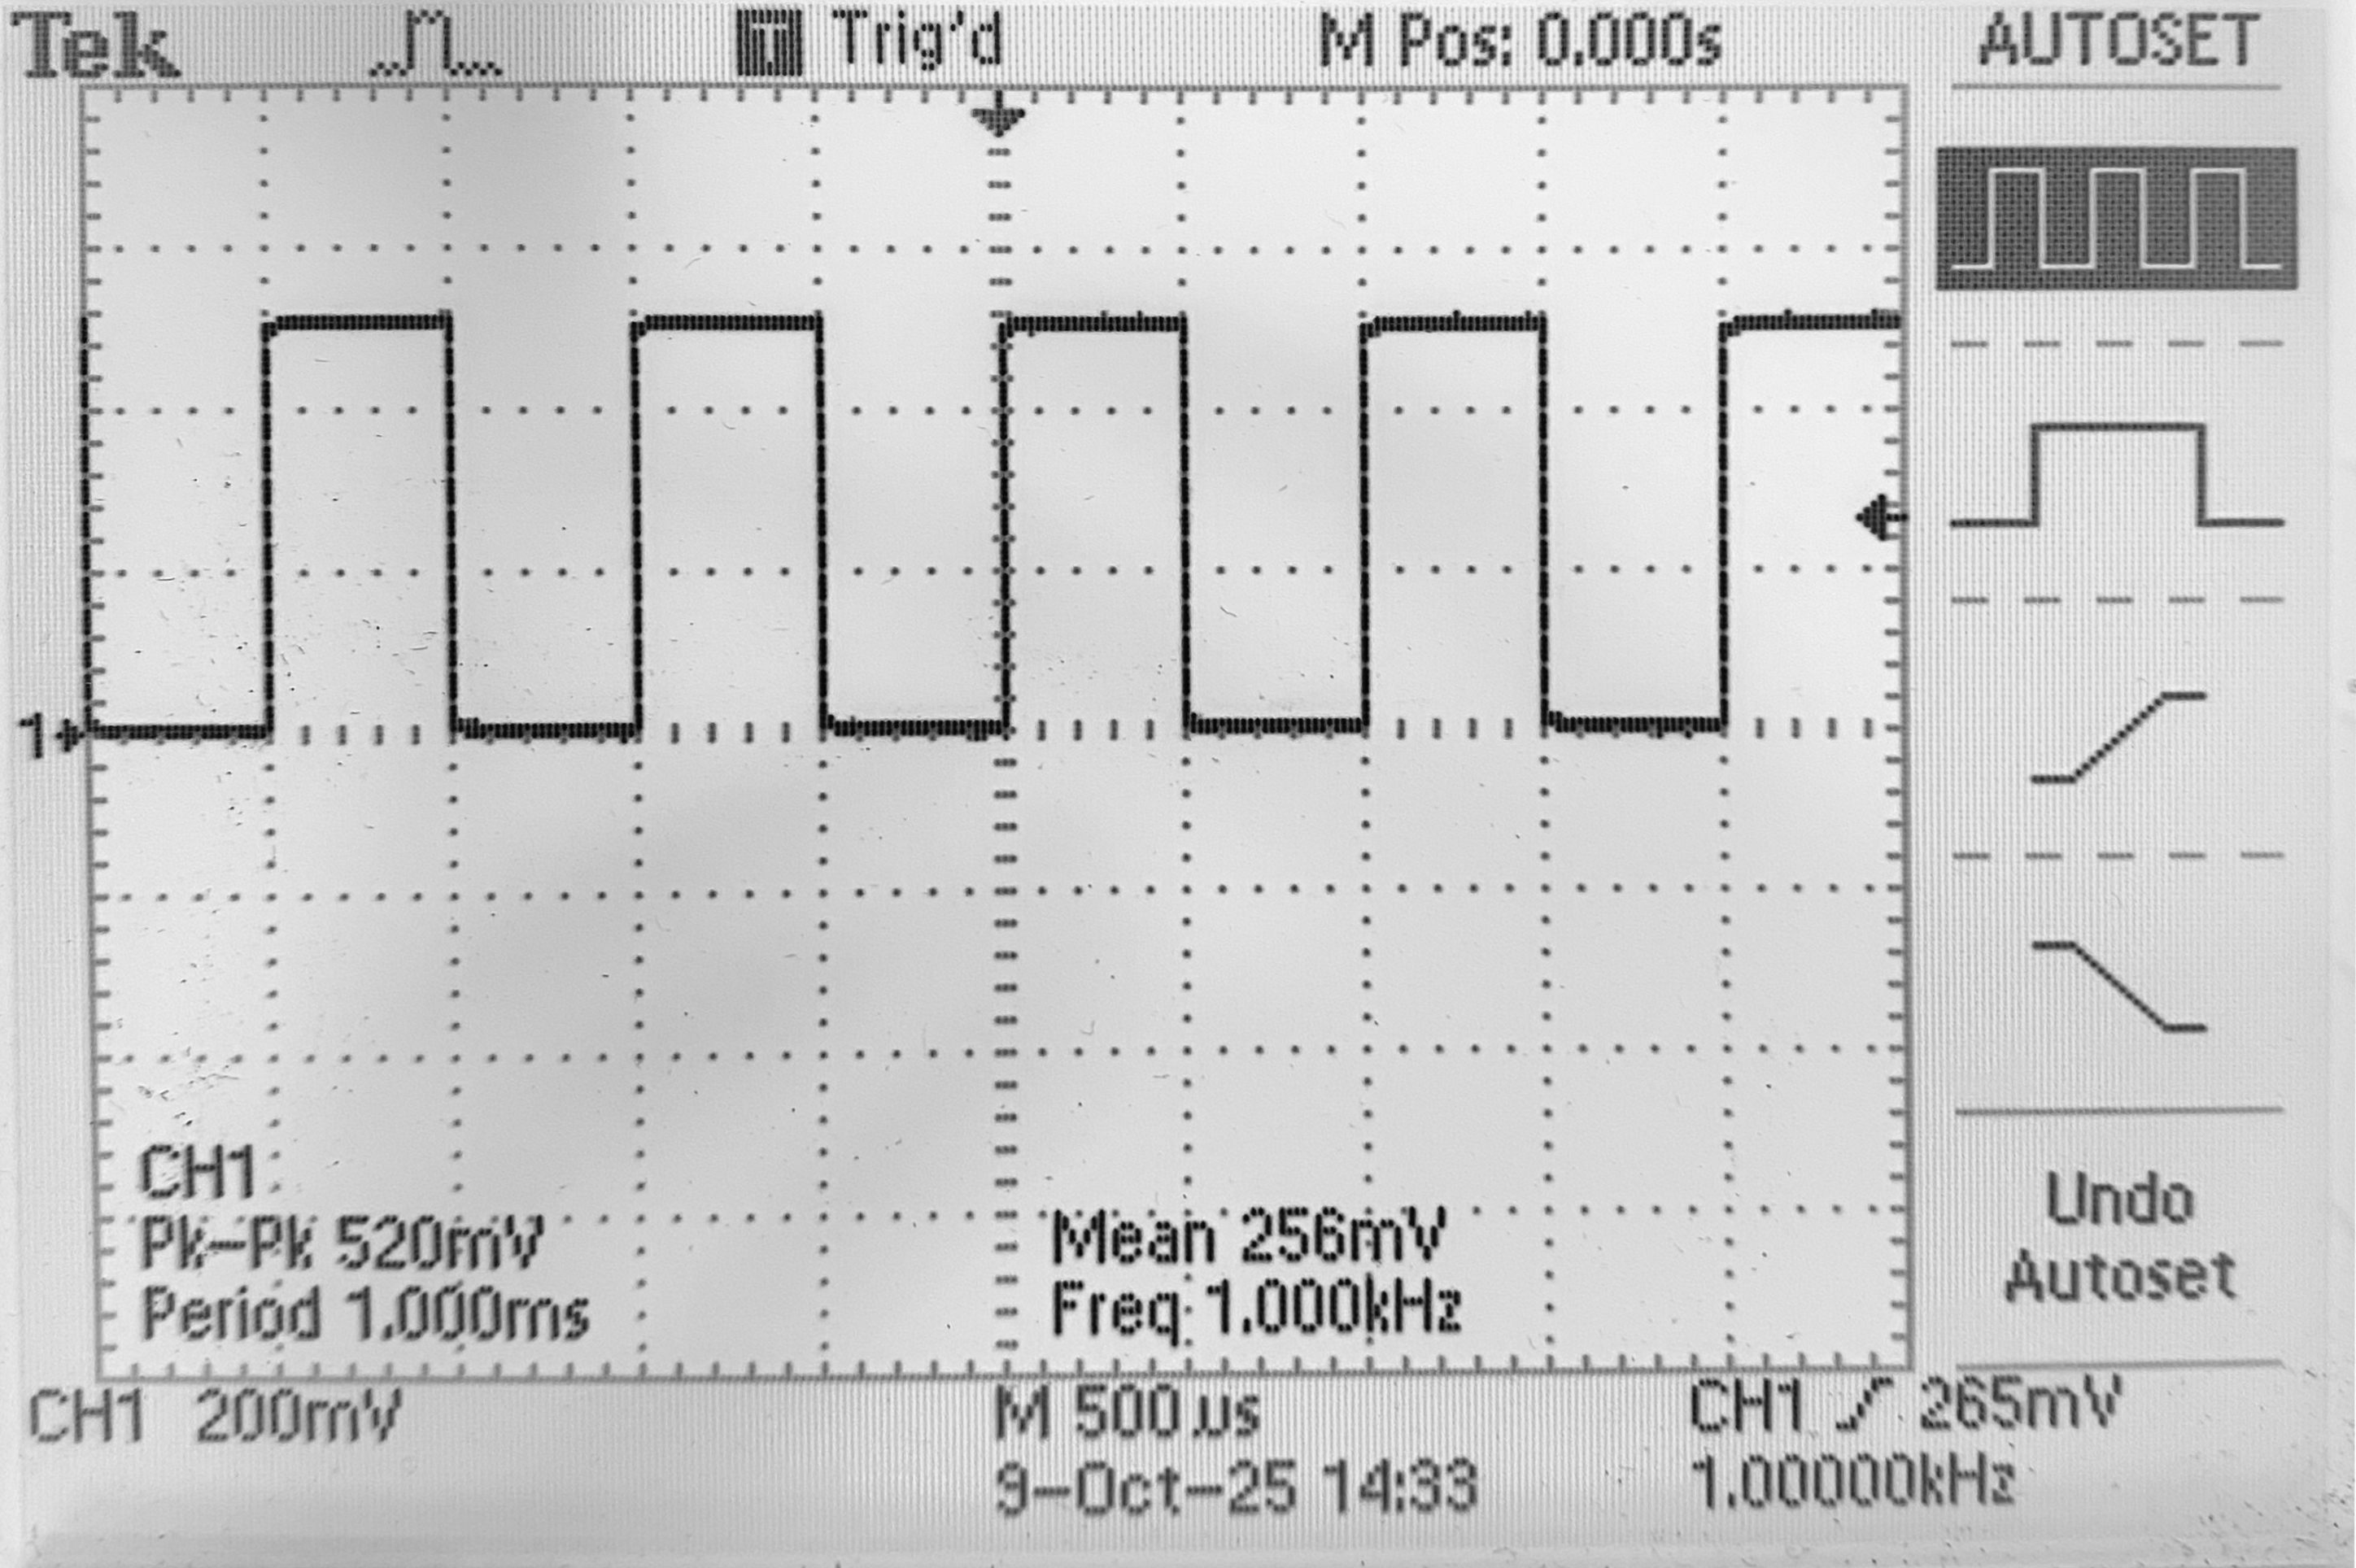
\includegraphics[height=4.8cm]{images/TastkopCal.JPEG}
		\caption{Abgleich eines Tastkopfes am Oszilloskop mittels Testsignal}\label{fig:oszi-tastkopf-testsignal}
	\end{minipage}\hfill
	\begin{minipage}[t]{.48\textwidth}
		\centering
		\begin{circuitikz}[scale=0.75, transform shape]
			% Eingangsspannung
			\draw (0,0) node[ocirc]{}
			(0,4) node[ocirc]{};
			\draw[<-] (0,0.3) -- (0,3.7) node[midway,left]{$U_E$};

			% Bauteile
			\draw (1,5) to[R, l=$R_{T}$] (3,5) coordinate (k1);
			\draw (1,3) to[variable capacitor, l=$C_{T}$] (3,3) coordinate (k2);
			\draw (5,0) to[C, l=$C_K$]   (5,4) coordinate (k3);
			\draw (7,0) to[C, l=$C_E$]   (7,4) coordinate (k4);
			\draw (9,0) to[R, l=$R_E$]   (9,4) coordinate (k5);

			% Kabel horizontal
			\draw (0,0) -- (9,0);
			\draw (0,4) -- (1,4);
			\draw (3,4) -- (9,4);
			% Kabel vertical
			\draw (1,3) -- (1,5);
			\draw (3,3) -- (3,5);
		\end{circuitikz}
		\captionof{figure}{Eingangsimpedanz des Oszilloskops bei AC-Kopplung}\label{fig:impedanz-oszi-taskopf}
	\end{minipage}
\end{figure}



\marginref{\ref{itm:2-P4-3}} Berechnung der Eingangsimpedanz bei 1 MHz

Aus der Abgleichbedinung $R_T C_T = R_E \tilde{C_E}$ kann man sich $C_T$ berechnen mit $\tilde{C_E} = C_E + C_K$.

\begin{align}
	 & C_T        = \frac{R_E}{R_T}(C_E + C_K) = \frac{\SI{1}{\mega\ohm}}{\SI{9}{\mega\ohm}}(\SI{20}{\pico\farad} + \SI{100}{\pico\farad}) = \SI{13.3}{\pico\farad} \\
	 & Z_{ges}    = Z_T + \tilde{Z_E} = \frac{R_T}{1+j\omega R_T C_T} + \frac{R_E}{1+j\omega R_E (C_k+C_E)} = \SI{17.67}{\ohm} - j\SI{13292.81}{\ohm}               \\
	 & |Z_{ges}|  = \SI{13292.82}{\ohm} \label{eq:eingangswiderstand_oszi_mit_taskopf}
\end{align}

\subsubsection{Erkenntnisse}
Mit dem Tastkopfe (Gl.~\ref{eq:eingangswiderstand_oszi_mit_taskopf}) ist $|Z_{ges}|$ ca. 10-mal so groß wie ohne (Gl.~\ref{eq:eingangswiderstand_oszi}). Dadurch ver-10-facht sich auch der Messbereich des Oszilloskops, was für große Signale notwendig ist. Allerdings verringert es auch die Empfindlichkeit was die Messung kleiner Signale ungenauer macht.


\newpage
\subsection{U-I-Kennlinien einer Silizium- und Zenerdiode}\label{sec:2-5}

\begin{highlightblock}[U-I-Kennlinien einer Silizium- und Zenerdiode]
	\begin{enumerate}[label=\textbf{\alph*:}, ref=\alph*]
		\item\label{itm:2-P5-1} Stellen Sie die UI-Kennlinie einer Silizium- und einer Zenerdiode dar.
		\item\label{itm:2-P5-2} Dimensionieren der Messspannungen und Vorwiderstände
		\item\label{itm:2-P5-3} Skizze inklusive Spannungs- und Strommaßstab des Schirmbildes.
		\item\label{itm:2-P5-4} Bestimmen Sie Knick- und Zenerspannung
		\item\label{itm:2-P5-5} Unterschied zwischen den beiden Kennlinien diskutieren.
	\end{enumerate}

\end{highlightblock}

\subsubsection{Verwendetes Material}

\begin{table}[h]
	\centering
	\caption{Verwendetes Material}
	\begin{tabularx}{\textwidth}{XXX}
		\textbf{Messgerät} & \textbf{Verwendung} & \textbf{Anmerkungen}                                \\ \midrule
		TDS2014C           & Oszilloskop         & $Z_E = \SI{1}{\mega\ohm}\,||\,\SI{20}{\pico\farad}$ \\
	\end{tabularx}
\end{table}

\subsubsection{Versuchsaufbau}

\begin{figure}[h]
	\begin{minipage}[t]{.98\textwidth}
		\centering
		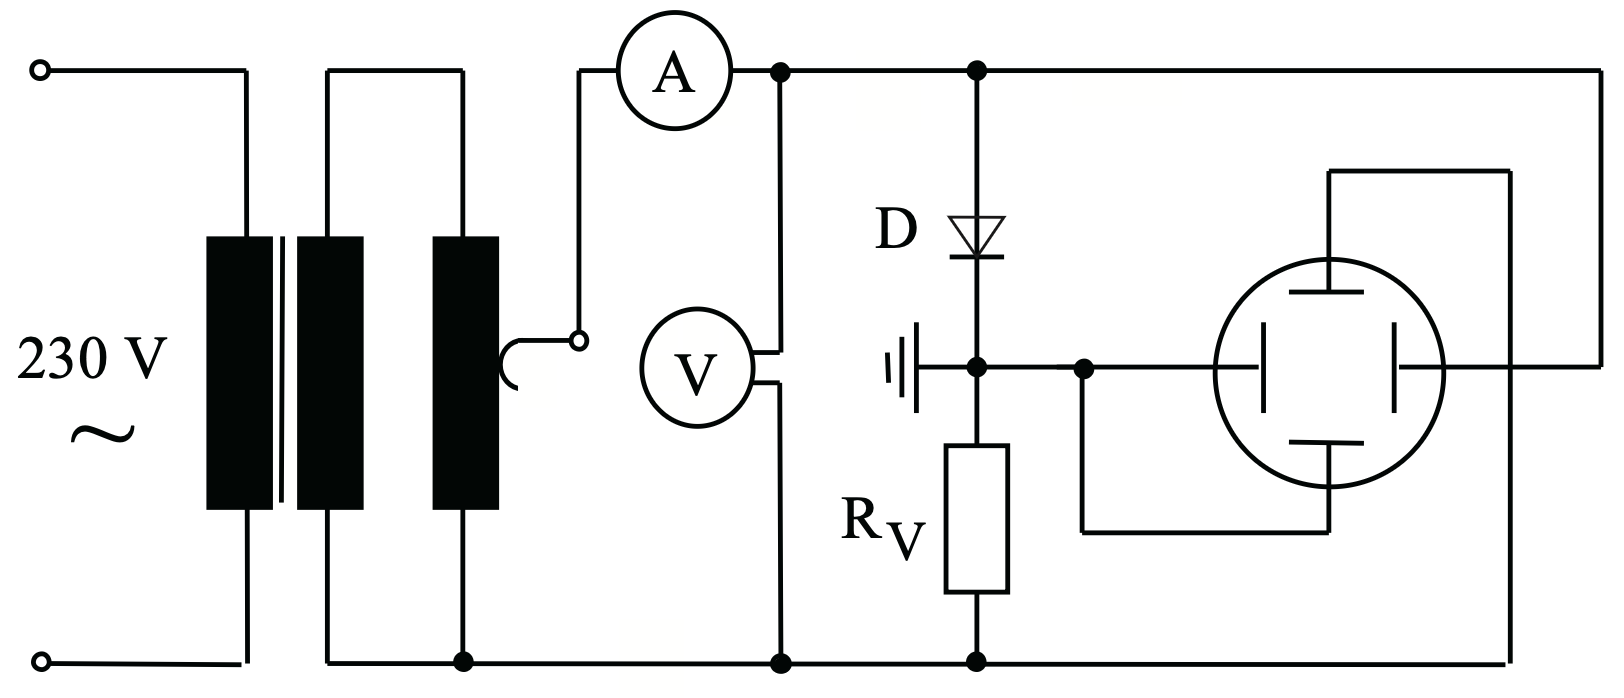
\includegraphics[height=4cm]{images/Schaltung-dioden-kennlinie.png}
		\caption{Abgleich eines Tastkopfes am Oszilloskop mittels Testsignal}\label{fig:schaltung-dioden-kennlinie.png}
	\end{minipage}\hfill
\end{figure}


\marginref{\ref{itm:2-P5-1}}

\marginref{\ref{itm:2-P5-2}}

\marginref{\ref{itm:2-P5-3}}

\marginref{\ref{itm:2-P5-4}}

\marginref{\ref{itm:2-P5-5}}

\subsubsection{Erkenntnisse}


\newpage
\subsection{Name des Aufbaus}\label{sec:2-6}

\begin{highlightblock}[Kurze Beschreibung des Aufbaus]
	Todo liste
	\begin{enumerate}[label=\textbf{\alph*:}, ref=\alph*]
		\item\label{itm:2-P6-1}
		\item\label{itm:2-P6-2}
		\item\label{itm:2-P6-3}
	\end{enumerate}

\end{highlightblock}

\subsubsection{Verwendetes Material}

\begin{table}[h]
	\centering
	\caption{Verwendetes Material}
	\begin{tabularx}{\textwidth}{XXX}
		\textbf{Messgerät} & \textbf{Verwendung} & \textbf{Anmerkungen} \\ \midrule
		                   &                     &                      \\
		                   &                     &                      \\
		                   &                     &                      \\
	\end{tabularx}
\end{table}

\subsubsection{Versuchsaufbau}

\begin{gather}
	U_{PP}/2=\SI{2.5}{\volt}
	\frac{\SI{2.5}{\volt}}{\SI{16}{\ohm}+R} < \SI{0.5}{\ampere} \\
	R=\SI{100}{\ohm} \\
	I = \frac{\SI{2.5}{\volt}}{\SI{16}{\ohm}+\SI{100}{\ohm}} \approx \SI{22}{\milli\ampere}
\end{gather}

\marginref{\ref{itm:2-P6-1}}
\marginref{\ref{itm:2-P6-2}}
\marginref{\ref{itm:2-P6-3}}

\subsubsection{Erkenntnisse}



\bibliographystyle{plain}
\bibliography{bib/literatur}


\end{document}
\endinput
